\documentclass[11pt, a4paper]{article}

% ─── PAQUETES ─────────────────────────────────────────────────────────────────
\usepackage[utf8]{inputenc}
\usepackage[T1]{fontenc}
\usepackage[spanish,es-tabla,es-noshorthands]{babel}
\usepackage{geometry}
\geometry{top=2.4cm, bottom=2.4cm, left=2.6cm, right=2.6cm, headheight=15pt}

\usepackage{amsmath, amssymb}
\usepackage{graphicx}
\usepackage{booktabs}
\usepackage{array}
\usepackage{multirow}
\usepackage{xcolor}
\usepackage{hyperref}
\usepackage{float}
\usepackage{caption}
\usepackage{enumitem}
\usepackage{fancyhdr}
\usepackage{titlesec}
\usepackage{parskip}
\usepackage{tikz}
\usetikzlibrary{arrows.meta, positioning}

\captionsetup{font=small, labelfont=bf}
\setlist{nosep, leftmargin=1.2em}

% ─── COLORES ──────────────────────────────────────────────────────────────────
\definecolor{azuloscuro}{RGB}{13, 71, 161}
\definecolor{azulclaro}{RGB}{227, 242, 253}

\hypersetup{colorlinks=true, linkcolor=azuloscuro, citecolor=azuloscuro, urlcolor=azuloscuro}

% ─── ENCABEZADO ───────────────────────────────────────────────────────────────
\pagestyle{fancy}
\fancyhf{}
\fancyhead[L]{\small\textcolor{azuloscuro}{\textbf{Redes bayesianas gaussianas y enfermedad renal crónica}}}
\fancyhead[R]{\small\textcolor{azuloscuro}{CKD -- UCI}}
\fancyfoot[C]{\thepage}
\renewcommand{\headrulewidth}{0.5pt}

% ─── SECCIONES ────────────────────────────────────────────────────────────────
\titleformat{\section}{\large\bfseries\color{azuloscuro}}{\thesection.}{0.5em}{}[\color{azuloscuro}\titlerule]
\titleformat{\subsection}{\normalsize\bfseries\color{azuloscuro!80}}{\thesubsection.}{0.5em}{}
\titlespacing*{\section}{0pt}{1.2ex}{0.8ex}
\titlespacing*{\subsection}{0pt}{1ex}{0.5ex}

\begin{document}

% ╔══════════════════════════════════════════════════════════════════════════════╗
\begin{center}
    \vspace*{0.3cm}
    {\LARGE\bfseries\color{azuloscuro}
        Redes Bayesianas Gaussianas para la\\[0.2em]
        Enfermedad Renal Crónica\par}
    \vspace{0.5em}
    \rule{0.85\textwidth}{1pt}\\[0.4em]
    {\large\itshape Estructuras elicitadas de especialistas, imputación por ecuaciones
    encadenadas y los límites del supuesto gaussiano en marcadores de laboratorio\par}
    \vspace{0.8em}
    {\normalsize
    Juan Pablo Venegas Padilla \quad\textbullet\quad Arie Zalo González\\[0.25em]
    Santiago de la Calleja Jiménez \quad\textbullet\quad Juan Pablo Espinoza\par}
    \vspace{0.3em}
    {\small Ingeniería en Ciencia de Datos y Matemáticas, Tecnológico de Monterrey
    \quad\textbullet\quad \today\par}
    \vspace{0.8em}
    \colorbox{azulclaro}{%
        \parbox{0.92\textwidth}{\small
            \vspace{0.2cm}
            \textbf{Resumen.} Este trabajo construye y evalúa \textbf{redes bayesianas gaussianas}
            (GBN) sobre 13 marcadores de laboratorio del dataset de \textbf{Enfermedad Renal
            Crónica} del repositorio UCI ($N=400$). A diferencia de los estudios que aprenden la
            estructura de los datos, aquí las estructuras se \textbf{elicitan de especialistas}:
            se entrevistó a tres estudiantes de Medicina, cada uno propuso un grafo de dependencias
            y dos consultas de interés clínico. La metodología encadena limpieza y clasificación de
            variables, \textbf{imputación por ecuaciones encadenadas} (MICE) con el diagnóstico
            como variable auxiliar —los faltantes llegan a 49.6\,\% en pacientes enfermos contra
            4.7\,\% en sanos, de modo que descartar filas sesgaría la muestra—, ajuste de una GBN
            por estructura, comparación por BIC y AIC, y respuesta a las seis consultas por
            muestreo lógico. La \textbf{DAG 2} resulta la mejor por ambos criterios
            (BIC $=-16{,}374.2$), y la diferencia decisiva es dónde cuelga la anemia: los datos
            favorecen hacerla depender de los marcadores de filtrado y no de los electrolitos, lo
            que coincide con que la eritropoyetina la produce el riñón. La red acierta el
            \textbf{sentido} de las seis consultas, pero no su magnitud, y este trabajo
            \textbf{cuantifica por qué}: solo 1 de 13 variables pasa la prueba de Shapiro--Wilk,
            el error relativo de cada consulta correlaciona con la asimetría de las variables
            implicadas ($\rho_{\text{Spearman}} = 0.898$, $p = 0.006$), y al condicionar sobre una
            cola la gaussiana \textbf{atenúa el co-movimiento} de las demás variables: predice una
            urea de 87.6 donde el grupo real promedia 143.6. Se documenta además que una búsqueda
            voraz sobre los datos supera a las tres propuestas por 278 puntos de BIC, pero a costa
            de orientaciones clínicamente imposibles. El trabajo cierra con dos extensiones: se
            desarrolla cómo entran las \textbf{variables categóricas} —red gaussiana condicional,
            con la diabetes confirmada por los datos en la posición que la clínica le asignaba
            ($+120$ puntos de BIC) y el diagnóstico como raíz discreta ($+1{,}888$)— y se evalúa si
            los \textbf{modelos no paramétricos} mejoran los criterios de información: el
            estimador kernel mejora el BIC nominal hasta en $3{,}620$ puntos, pero ese número no es
            comparable y fuera de muestra la ventaja se desvanece; las ganancias reales vienen de
            una transformación monótona de las marginales más la mezcla condicional, que reducen el
            error medio de las consultas de $38.3$\,\% a $24.9$\,\%.
            \vspace{0.2cm}}}
    \vspace{0.4em}

    {\small\textbf{Palabras clave---} Redes bayesianas gaussianas, enfermedad renal crónica,
    elicitación de expertos, imputación múltiple, MICE, \texttt{bnlearn}, supuesto de normalidad,
    inferencia condicional.\par}
    \vspace{0.6em}
\end{center}

% ─── 1. INTRODUCCIÓN ──────────────────────────────────────────────────────────
\section{Introducción}

La enfermedad renal crónica (ERC) es un deterioro progresivo y en buena medida silencioso de la
función renal: cuando aparecen los síntomas, el daño suele estar avanzado \cite{levey2012}. Su
diagnóstico y seguimiento descansan en un puñado de marcadores de laboratorio —creatinina sérica,
urea, densidad urinaria, albuminuria, electrolitos y biometría hemática— cuyas relaciones los
clínicos conocen bien, pero que rara vez se formalizan en un modelo probabilístico conjunto.

Ese es el punto de partida de este trabajo. Los 400 pacientes del dataset de ERC del repositorio
UCI \cite{ckd2015} traen esos marcadores medidos, y las relaciones entre ellos son exactamente el
tipo de conocimiento que un modelo gráfico puede representar. La pregunta que organiza el estudio
no es si un algoritmo puede descubrir esa estructura, sino algo más cercano a la práctica clínica:
\textbf{si se le pide a un médico que dibuje cómo cree que se relacionan estas variables, ¿qué tan
bien se sostiene su dibujo frente a los datos, y qué tan lejos llegan las respuestas que se pueden
obtener de él?}

\subsection{Antecedentes y estado del arte}

Una red bayesiana codifica una distribución conjunta mediante un grafo acíclico dirigido (DAG) en
el que cada arco $A \rightarrow B$ afirma una dependencia directa \cite{pearl1988,koller2009}.
Cuando todas las variables son continuas y cada nodo se modela como una regresión lineal sobre sus
padres con residuo normal, la red se llama \textbf{gaussiana}: la distribución conjunta resultante
es una normal multivariada y sus parámetros se estiman por mínimos cuadrados
\cite{shachter1989,geiger1994}. Esta familia es atractiva porque el ajuste es cerrado y barato, y
porque cada arco tiene una lectura inmediata —un coeficiente de regresión— que un especialista
puede discutir.

Su precio es el supuesto. Una GBN obliga a cada variable a ser normal condicionalmente a sus
padres y a que toda dependencia sea lineal. Cuando los datos son marcadores de laboratorio —donde
lo clínicamente relevante suele estar justamente en la cola— ese supuesto es fuerte. La extensión
natural son las \textbf{redes gaussianas condicionales} (CLGBN) de Lauritzen y Wermuth
\cite{lauritzen1989,lauritzen1992}, que admiten nodos discretos siempre que no tengan padres
continuos. La implementación de referencia de ambas familias es el paquete \texttt{bnlearn}
\cite{scutari2010}, que provee el ajuste, los criterios de información de Akaike \cite{akaike1974}
y Schwarz \cite{schwarz1978}, y la inferencia aproximada por muestreo lógico.

En el ámbito biomédico, las redes bayesianas se han usado para diagnóstico, pronóstico y análisis
de dependencias entre hallazgos clínicos desde hace tres décadas \cite{lucas2004,kononenko2001}.
La elicitación de estructura con expertos, en particular, es un procedimiento reconocido cuando el
tamaño de muestra no alcanza para que el aprendizaje automático identifique orientaciones
confiables: el grafo aporta el conocimiento causal que los datos por sí solos no contienen.

El otro problema que este dataset impone es el de los datos faltantes. La distinción de Rubin
\cite{rubin1976} entre faltantes completamente al azar, al azar y no al azar es decisiva aquí:
como se documenta más abajo, la ausencia de dato está fuertemente asociada al diagnóstico, así
que eliminar registros incompletos vaciaría selectivamente el grupo enfermo. La imputación por
ecuaciones encadenadas \cite{vanbuuren2011,little2002} resuelve el problema con una lógica que,
además, coincide con la del modelo que se va a ajustar: cada variable se estima como una regresión
de las demás.

\subsection{Problema y preguntas de investigación}

Se entrevistó a tres personas de la Escuela de Medicina del campus —un estudiante de 5º semestre y
dos de 9º—. Cada una propuso una estructura de dependencias entre las 13 variables continuas y dos
consultas que le interesaría resolver con el modelo:

\begin{enumerate}
    \item[\textbf{C1}] $P(\text{creatinina} > 3 \mid \text{presión} \geq 90)$.
    \item[\textbf{C2}] $E[\text{hematocrito} \mid \text{hemoglobina} < 10]$.
    \item[\textbf{C3}] $E[\text{hemoglobina} \mid \text{creatinina} > 5]$.
    \item[\textbf{C4}] $P(\text{potasio} > 5.5 \mid \text{urea} > 100)$.
    \item[\textbf{C5}] $E[\text{albúmina} \mid \text{glucosa} < 140]$ frente a
        $E[\text{albúmina} \mid \text{glucosa} > 200]$.
    \item[\textbf{C6}] $P(\text{creatinina} > 3 \mid \text{diabetes})$.
\end{enumerate}

Las preguntas de investigación son tres: ¿cuál de las tres estructuras propuestas se ajusta mejor
a los datos y en qué difieren sustantivamente?; ¿qué respuestas produce la mejor red a las seis
consultas y qué tan cerca están de lo que muestran los datos?; y ¿cómo entra al modelo una
variable categórica como la diabetes, que una GBN pura no admite?

\subsection{Objetivos}

\textbf{General:} construir, comparar y validar redes bayesianas gaussianas sobre los marcadores
de laboratorio de la ERC a partir de estructuras elicitadas de especialistas, y responder con la
mejor de ellas las consultas clínicas planteadas. \textbf{Específicos:} (i)~limpiar el dataset y
separar las variables que una GBN admite de las que no; (ii)~imputar los faltantes con un método
compatible con el modelo y validar que la señal clínica se conserve; (iii)~formalizar las tres
estructuras y verificar su aciclicidad; (iv)~ajustarlas y compararlas por BIC y AIC;
(v)~responder las seis consultas y contrastarlas contra la evidencia empírica; y (vi)~diagnosticar
el supuesto gaussiano y cuantificar su efecto sobre las respuestas.

\subsection{Aportaciones}

\begin{enumerate}
    \item Un flujo \textbf{reproducible y auditable} que va del CSV crudo —con tokens de texto
        incrustados en columnas numéricas— a una base imputada lista para modelar, con la
        validación de que la imputación no desplaza las diferencias clínicas entre grupos.
    \item La \textbf{formalización de tres estructuras elicitadas de especialistas} y su
        comparación cuantitativa, incluyendo el caso de una relación clínicamente real —la
        retroalimentación de los electrolitos sobre la presión arterial— que un DAG no puede
        representar por ser cíclica.
    \item Un \textbf{diagnóstico cuantitativo del supuesto gaussiano} que explica, variable por
        variable y consulta por consulta, por qué la red acierta el sentido pero falla la
        magnitud: el error relativo correlaciona con la asimetría
        ($\rho = 0.898$, $p = 0.006$) y la condicional gaussiana atenúa el co-movimiento de las
        colas de forma medible.
    \item Un \textbf{contraste contra una búsqueda voraz} sobre los mismos datos, que gana 278
        puntos de BIC pero produce orientaciones imposibles —la edad como efecto del conteo de
        eritrocitos—, delimitando qué aporta el experto y qué aportan los datos.
    \item Un \textbf{estudio de la incorporación de variables categóricas}: la formalización de la
        red gaussiana condicional, la búsqueda de la mejor posición para la diabetes —que confirma
        la elección clínica y a la vez expone la fuga del diagnóstico—, el diagnóstico como raíz
        discreta y el costo medido de la alternativa de discretizar.
    \item Una \textbf{evaluación de nueve variantes no paramétricas y semiparamétricas} bajo tres
        criterios (BIC, AIC y verosimilitud fuera de muestra), que muestra por qué el BIC no es un
        criterio válido para componentes no paramétricos y qué relajaciones sí mejoran las
        respuestas del modelo.
\end{enumerate}

% ─── 2. METODOLOGÍA ───────────────────────────────────────────────────────────
\section{Metodología}

\subsection{Arquitectura del flujo de trabajo}

El proyecto se divide en dos etapas con lenguajes distintos. La \textbf{preparación} corre en
Python con \texttt{pandas} \cite{mckinney2010} y \texttt{scikit-learn} \cite{pedregosa2011} sobre
dos cuadernos —análisis exploratorio e imputación— y produce un único archivo,
\texttt{ckd\_imputado.csv}. El \textbf{modelado} corre en R con \texttt{bnlearn}
\cite{scutari2010,rcore2024} sobre dos documentos Quarto: uno que formaliza las estructuras
elicitadas y otro que las ajusta y responde las consultas. La Fig.~\ref{fig:metodologia} resume
las cinco fases. Todo el código está disponible en
\url{https://github.com/JuanPabloEspTEC/MRI-art_2-RBG}.

\begin{figure}[H]
\centering
\begin{tikzpicture}[
    block/.style={rectangle, draw=azuloscuro, thick, fill=white, text width=11cm,
                  minimum height=0.95cm, align=left, rounded corners=2pt, font=\small},
    arrow/.style={-{Stealth[scale=1.1]}, thick, azuloscuro}
]
\node (s1) [block] {\textbf{1. Análisis exploratorio y limpieza}\\
    Tipos, niveles espurios, separación entre variables continuas y discretas.};
\node (s2) [block, below=0.42cm of s1] {\textbf{2. Imputación de faltantes}\\
    MICE con el diagnóstico como variable auxiliar; validación por grupo.};
\node (s3) [block, below=0.42cm of s2] {\textbf{3. Elicitación de estructuras}\\
    Tres entrevistas en la Escuela de Medicina; tres DAGs y seis consultas.};
\node (s4) [block, below=0.42cm of s3] {\textbf{4. Ajuste y comparación}\\
    Una GBN por estructura (\texttt{mle-g}), BIC-g, AIC-g y \texttt{arc.strength}.};
\node (s5) [block, below=0.42cm of s4] {\textbf{5. Inferencia y diagnóstico}\\
    \texttt{cpquery}/\texttt{cpdist}, contraste empírico y prueba del supuesto gaussiano.};
\draw [arrow] (s1) -- (s2);
\draw [arrow] (s2) -- (s3);
\draw [arrow] (s3) -- (s4);
\draw [arrow] (s4) -- (s5);
\end{tikzpicture}
\caption{Metodología propuesta, en cinco fases secuenciales.}
\label{fig:metodologia}
\end{figure}

\subsection{Datos y limpieza}

El dataset de ERC del repositorio UCI \cite{ckd2015} reúne \textbf{400 pacientes} y 25 variables
—24 atributos más el diagnóstico— recolectados en un hospital a lo largo de aproximadamente dos
meses. El diagnóstico está desbalanceado: \textbf{250 casos \texttt{ckd}} contra
\textbf{150 \texttt{notckd}} (62.5\,\% / 37.5\,\%).

La inspección inicial detectó cuatro problemas, resumidos en la Tabla~\ref{tab:limpieza}. El más
insidioso es el tercero: \texttt{pcv}, \texttt{wc} y \texttt{rc} son conteos hematológicos, pero
llegaban como texto porque algunas celdas contenían el token \verb|'\t?'|. Leídas así, esas tres
variables quedan fuera de cualquier cálculo numérico sin que nada lo advierta; convertidas
correctamente, el token pasa a contarse como el dato faltante que en realidad es.

\begin{table}[H]
\centering
\caption{Problemas detectados en el archivo original y acción tomada.}
\label{tab:limpieza}
\small
\renewcommand{\arraystretch}{1.15}
\begin{tabular}{p{7.2cm} p{7.2cm}}
\toprule
\textbf{Problema} & \textbf{Acción} \\
\midrule
\texttt{id} tiene 400 valores únicos: es un identificador, no una variable. & Se elimina la columna. \\
\texttt{classification} reporta 3 niveles cuando el diagnóstico solo puede ser \texttt{ckd} o \texttt{notckd}; \texttt{dm} reporta 5 y \texttt{cad} 3. & Se normaliza el texto (espacios y tabuladores); quedan 2 niveles en cada una. \\
\texttt{pcv}, \texttt{wc} y \texttt{rc} son numéricas pero pandas las lee como texto por el token \verb|'\t?'|. & Se convierten a \texttt{float64}; el token pasa a contarse como faltante. \\
Los faltantes no son menores: \texttt{rbc} 38\,\%, \texttt{rc} 32.5\,\%, \texttt{wc} 26.3\,\%. & Se analizan por grupo diagnóstico antes de decidir la estrategia (\S2.4). \\
\bottomrule
\end{tabular}
\end{table}

\subsection{Qué variables admite una red gaussiana}

Esta es la decisión que condiciona todo lo demás: \textbf{una red bayesiana gaussiana solo admite
variables continuas}. De las 25 columnas, 11 son categóricas y una más (\texttt{su}, azúcar en
orina) es un conteo ordinal de seis niveles, de modo que \textbf{13 variables} quedan disponibles
para el modelo: \texttt{age}, \texttt{bp}, \texttt{sg}, \texttt{al}, \texttt{bgr}, \texttt{bu},
\texttt{sc}, \texttt{sod}, \texttt{pot}, \texttt{hemo}, \texttt{pcv}, \texttt{wc} y \texttt{rc}.
El propio diagnóstico queda fuera de las estructuras, y en \S3.5 se muestra cómo reincorporarlo.

Conviene dejar asentada una tensión que el análisis exploratorio ya señalaba. Tres de esas 13
variables son, estrictamente, ordinales o redondeadas: \texttt{bp} se registró en múltiplos de 10 y
toma 10 valores distintos, \texttt{sg} toma 5 y \texttt{al} toma 6. Se conservan como continuas
—sin ellas la cascada clínica se rompe—, pero su naturaleza discreta reaparece en el diagnóstico
del supuesto gaussiano de \S3.7.

\subsection{Faltantes e imputación}

El patrón de faltantes no es aleatorio. La Tabla~\ref{tab:variables} lo muestra desglosado por
diagnóstico: en \texttt{rc} falta el \textbf{49.6\,\%} de los datos entre pacientes enfermos y
apenas el \textbf{4.7\,\%} entre sanos, y el mismo contraste se repite en todas las variables. La
lectura clínica es transparente —a un paciente sano no se le piden los mismos estudios que a uno
en protocolo de ERC—, pero la consecuencia estadística es seria: solo \textbf{203 de 400} filas
están completas en las 13 continuas (158 si se exigen las 25 variables), y descartar las
incompletas vaciaría selectivamente el grupo enfermo. Es un caso de libro de faltantes no
aleatorios \cite{rubin1976}, donde el análisis de casos completos sesga.

\begin{table}[H]
\centering
\caption{Las 13 variables continuas del modelo y su porcentaje de faltantes, desglosado por
diagnóstico.}
\label{tab:variables}
\small
\renewcommand{\arraystretch}{1.12}
\begin{tabular}{l l r r r}
\toprule
\textbf{Variable} & \textbf{Significado} & \textbf{\% total} & \textbf{\% \texttt{ckd}} & \textbf{\% \texttt{notckd}} \\
\midrule
\texttt{rc}   & Eritrocitos        & 32.8 & 49.6 & 4.7 \\
\texttt{wc}   & Leucocitos         & 26.5 & 39.6 & 4.7 \\
\texttt{pot}  & Potasio sérico     & 22.0 & 33.2 & 3.3 \\
\texttt{sod}  & Sodio sérico       & 21.8 & 32.8 & 3.3 \\
\texttt{pcv}  & Hematocrito        & 17.8 & 26.8 & 2.7 \\
\texttt{hemo} & Hemoglobina        & 13.0 & 18.4 & 4.0 \\
\texttt{sg}   & Densidad urinaria  & 11.8 & 16.8 & 3.3 \\
\texttt{al}   & Albúmina en orina  & 11.5 & 16.4 & 3.3 \\
\texttt{bgr}  & Glucosa en sangre  & 11.0 & 15.2 & 4.0 \\
\texttt{bu}   & Urea en sangre     &  4.8 &  5.2 & 4.0 \\
\texttt{sc}   & Creatinina sérica  &  4.2 &  4.8 & 3.3 \\
\texttt{bp}   & Presión arterial   &  3.0 &  4.0 & 1.3 \\
\texttt{age}  & Edad               &  2.2 &  3.2 & 0.7 \\
\bottomrule
\end{tabular}
\end{table}

Se evaluaron tres alternativas. La imputación por media o mediana es simple pero ignora la
relación entre variables y reduce artificialmente la varianza. El vecino más cercano (KNN)
considera la similitud entre pacientes pero es muy sensible a la escala, y aquí las escalas van de
$1.02$ (densidad urinaria) a $8{,}400$ (leucocitos). Se eligió \textbf{MICE}
(\texttt{IterativeImputer}, \texttt{random\_state}~$=42$, \texttt{max\_iter}~$=15$) por una razón
de fondo: su lógica es la misma que la del modelo que se va a ajustar —cada variable como
combinación lineal de las demás bajo supuesto gaussiano—, de modo que la imputación no introduce
una estructura ajena a la red \cite{vanbuuren2011}. Como los faltantes dependen del diagnóstico,
este se incluyó codificado como $0/1$ durante la imputación y se descartó al terminar.

\subsection{Redes bayesianas gaussianas}

Sea $\mathbf{X}=(X_1,\ldots,X_p)$ un vector de variables continuas y $\mathcal{G}$ un DAG sobre
ellas. La red factoriza la conjunta según la estructura del grafo,
\begin{equation}
    f(x_1,\ldots,x_p) = \prod_{i=1}^{p} f\bigl(x_i \mid \mathrm{pa}(x_i)\bigr),
    \label{eq:factorizacion}
\end{equation}
y en el caso gaussiano cada factor es una regresión lineal con residuo normal:
\begin{equation}
    X_i \mid \mathrm{pa}(X_i) \;\sim\; \mathcal{N}\!\Bigl(\beta_{i0} +
    \!\!\sum_{X_j \in \mathrm{pa}(X_i)}\!\! \beta_{ij} X_j,\; \sigma_i^2\Bigr).
    \label{eq:gbn}
\end{equation}
Ajustar la red es, por tanto, estimar para cada nodo un intercepto, un coeficiente por padre y la
desviación estándar de los residuos; con \texttt{method = "mle-g"} esto se resuelve por mínimos
cuadrados ordinarios nodo por nodo \cite{shachter1989,geiger1994}. La conjunta resultante es una
normal multivariada cuya matriz de covarianzas queda determinada por los coeficientes y las
varianzas residuales.

La comparación entre estructuras usa los dos criterios de información en su versión gaussiana, en
la convención de \texttt{bnlearn} donde un valor \textbf{mayor} indica mejor ajuste:
\begin{align}
    \mathrm{BIC}(\mathcal{G}) &= \log \hat{L}(\mathcal{G}) - \frac{\log n}{2}\,|\Theta_{\mathcal{G}}|,
    \label{eq:bic}\\
    \mathrm{AIC}(\mathcal{G}) &= \log \hat{L}(\mathcal{G}) - |\Theta_{\mathcal{G}}|,
    \label{eq:aic}
\end{align}
donde $|\Theta_{\mathcal{G}}| = \sum_i \bigl(|\mathrm{pa}(X_i)| + 2\bigr)$ cuenta interceptos,
coeficientes y desviaciones residuales. Para medir el aporte de cada arco se usa
\texttt{arc.strength} con criterio \texttt{bic-g}, que reporta \textbf{el cambio en el BIC si el
arco se elimina}: un valor negativo significa que quitarlo empeora el modelo —el arco está
sostenido por los datos— y uno positivo, que sobra.

\subsection{Inferencia}

Las consultas se responden con \texttt{cpquery} (probabilidades) y \texttt{cpdist} (valores
esperados sobre la distribución condicional simulada), ambas por \textbf{muestreo lógico}: se
generan realizaciones de la red, se descartan las incompatibles con la evidencia y se calcula la
proporción o el promedio sobre las restantes. Se usan $10^6$ muestras para las probabilidades y
$10^5$ para las esperanzas, con semilla fija (\texttt{set.seed(42)}). Cada respuesta se acompaña
de la frecuencia observada en los datos, calculada sobre el mismo universo, como referencia.

\subsection{Cómo entran las variables categóricas}
\label{sec:met-categoricas}

Ni el diagnóstico ni la diabetes son continuos, de modo que ninguno cabe en una GBN pura. La
literatura ofrece tres caminos, con costos distintos.

\textbf{(a) Red gaussiana condicional (CLGBN).} Es la extensión canónica del modelo gaussiano a
variables mixtas \cite{lauritzen1989,lauritzen1992}. Se parte el conjunto de nodos en discretos
$\mathbf{D}$ y continuos $\mathbf{Y}$, y la conjunta se escribe como el producto de una
distribución discreta por una gaussiana \textit{condicionada a la configuración discreta}:
\begin{equation}
    f(\mathbf{d},\mathbf{y}) = p(\mathbf{d}) \prod_{Y_i \in \mathbf{Y}}
    \mathcal{N}\!\Bigl(y_i \;\Big|\; \beta_{i0}^{(\mathbf{d}_i)} +
    \!\!\!\sum_{Y_j \in \mathrm{pa}_c(Y_i)}\!\!\! \beta_{ij}^{(\mathbf{d}_i)} y_j,\;
    \bigl(\sigma_i^{(\mathbf{d}_i)}\bigr)^2\Bigr),
    \label{eq:clgbn}
\end{equation}
donde $\mathbf{d}_i$ es la configuración de los padres discretos de $Y_i$ y
$\mathrm{pa}_c(Y_i)$ sus padres continuos. En palabras: \textbf{cada nodo continuo tiene una
regresión distinta por cada combinación de sus padres discretos}. La restricción del formalismo es
que \textbf{un nodo discreto no puede tener padres continuos}, y la razón es estructural, no
computacional: si un nodo discreto dependiera de uno continuo, la marginal del continuo dejaría de
ser una mezcla finita de gaussianas y la familia perdería el cierre que hace tratable la
inferencia. El costo en parámetros es multiplicativo: un nodo continuo con $k$ padres continuos y
padres discretos con $|\mathbf{d}_i|$ configuraciones pasa de $k+2$ a $|\mathbf{d}_i|(k+2)$
parámetros.

\textbf{(b) Discretizar todo y usar una red multinomial.} Funciona con cualquier combinación de
variables y es la opción del artículo anterior de esta serie, pero paga el precio de agrupar en
intervalos: en un marcador con cola larga, casi toda la masa cae en el primer intervalo y la
variable se vuelve, en la práctica, constante (\S3.6.4 lo cuantifica).

\textbf{(c) Codificar la categoría como $0/1$} y tratarla como continua. Es la más fácil y la menos
defendible: le asigna una distancia numérica a algo que no la tiene, obliga a una binaria a ser
normal y, en la inferencia, produce valores intermedios sin interpretación —¿qué es un paciente con
diabetes $=0.4$?—.

Se adoptó la primera. La \S3.6 la desarrolla: dónde conviene colocar la variable discreta según
los datos, qué pasa cuando el discreto es el propio diagnóstico y cuánto cuesta cada alternativa.

\subsection{Modelos no paramétricos y semiparamétricos}
\label{sec:met-noparam}

La segunda pregunta de este trabajo es si relajar el supuesto gaussiano —el que \S3.8 muestra
violado— mejora el ajuste medido por BIC y AIC. Conviene precisar qué significa ``no paramétrico''
dentro de una red bayesiana, porque hay al menos cuatro familias:

\begin{enumerate}
    \item \textbf{CPD por estimación de densidad kernel.} Se conserva el DAG pero la densidad
        condicional de cada nodo se estima con un núcleo en lugar de una normal
        \cite{hofmann1996,silverman1986}. Es la opción más flexible y la que menos supuestos hace.
    \item \textbf{Redes bayesianas semiparamétricas.} Cada nodo elige entre una CPD lineal
        gaussiana y una CPD por kernel condicional, y la elección se hace por
        \textbf{verosimilitud validada cruzadamente} \cite{atienza2022}. Es el punto medio entre
        (1) y el modelo gaussiano.
    \item \textbf{Transformaciones monótonas de las marginales.} La familia nonparanormal o de
        cópula gaussiana \cite{liu2009,elidan2010} transforma cada variable para que su marginal
        sea normal y conserva la estructura gaussiana en el espacio transformado. Sus versiones
        paramétricas son las transformaciones de potencia de Box--Cox \cite{box1964} y
        Yeo--Johnson \cite{yeo2000}, que admiten zeros y valores negativos.
    \item \textbf{Mezclas de exponenciales truncadas o de polinomios} (MTE, MOP)
        \cite{moral2001,shenoy2011}, que aproximan cualquier densidad por trozos manteniendo la
        propagación exacta.
\end{enumerate}

Aquí aparece un problema de método que conviene declarar antes de reportar cualquier número.
\textbf{El BIC no está definido para un componente no paramétrico.} La derivación de Schwarz
\cite{schwarz1978} supone una familia paramétrica de dimensión fija, y la penalización
$\tfrac{1}{2}\log n \cdot |\Theta|$ cuenta esos parámetros; un estimador kernel no tiene un
$|\Theta|$ que contar —sus grados de libertad efectivos crecen con $n$— de modo que aplicarle la
fórmula subestima su complejidad y sesga la comparación a su favor. Por eso la literatura
semiparamétrica \cite{atienza2022,hastie2009} selecciona por \textbf{verosimilitud fuera de
muestra}. En \S3.9 se reportan las tres cifras —BIC nominal, AIC nominal y log-verosimilitud
validada cruzadamente en 5 particiones— y se muestra que llevan a conclusiones distintas.

Dos precisiones técnicas más. Primero, comparar modelos ajustados sobre datos transformados exige
\textbf{devolver la verosimilitud a la escala original} sumando el logaritmo del jacobiano de la
transformación; sin esa corrección, cualquier transformación que comprima la escala ``mejora'' el
puntaje de manera espuria. Para Yeo--Johnson con $x \geq 0$ el jacobiano es
$(\lambda-1)\sum_i \log(x_i+1)$, y los $\lambda$ estimados por máxima verosimilitud se cuentan como
parámetros adicionales. Segundo, la verosimilitud de los modelos con kernel se calcula
\textbf{dejando fuera el propio punto} (\textit{leave-one-out}), para que la densidad de cada
observación no esté inflada por su propia contribución.

% ─── 3. APLICACIÓN ────────────────────────────────────────────────────────────
\section{Aplicación y resultados}

\subsection{Imputación y validación}

Tras la imputación, la base queda en \textbf{400 filas $\times$ 13 columnas sin un solo faltante}.
La validación consistió en comparar las medias por grupo diagnóstico antes y después
(Tabla~\ref{tab:imputacion}): si la imputación hubiera desplazado el centro de las distribuciones o
diluido las diferencias clínicas, no serviría como insumo del modelo.

\begin{table}[H]
\centering
\caption{Medias por grupo diagnóstico antes y después de imputar. Las diferencias clínicas se
conservan.}
\label{tab:imputacion}
\small
\renewcommand{\arraystretch}{1.1}
\begin{tabular}{l r r c r r}
\toprule
& \multicolumn{2}{c}{\textbf{\texttt{ckd}} ($n=250$)} & &
  \multicolumn{2}{c}{\textbf{\texttt{notckd}} ($n=150$)} \\
\cmidrule(lr){2-3}\cmidrule(lr){5-6}
\textbf{Variable} & \textbf{antes} & \textbf{después} & & \textbf{antes} & \textbf{después} \\
\midrule
\texttt{age}  &   54.54 &   54.48 & &   46.52 &   46.53 \\
\texttt{bp}   &   79.62 &   79.46 & &   71.35 &   71.36 \\
\texttt{sg}   &    1.01 &    1.01 & &    1.02 &    1.02 \\
\texttt{al}   &    1.72 &    1.76 & &    0.00 &    0.00 \\
\texttt{bgr}  &  175.42 &  172.37 & &  107.72 &  108.59 \\
\texttt{bu}   &   72.39 &   72.08 & &   32.80 &   32.82 \\
\texttt{sc}   &    4.41 &    4.34 & &    0.87 &    0.92 \\
\texttt{sod}  &  133.90 &  134.63 & &  141.73 &  141.71 \\
\texttt{pot}  &    4.88 &    4.68 & &    4.34 &    4.33 \\
\texttt{hemo} &   10.65 &   10.82 & &   15.19 &   15.17 \\
\texttt{pcv}  &   32.94 &   33.29 & &   46.34 &   46.32 \\
\texttt{wc}   & 9069.54 & 8841.66 & & 7705.59 & 7730.67 \\
\texttt{rc}   &    3.95 &    4.06 & &    5.38 &    5.37 \\
\bottomrule
\end{tabular}
\end{table}

Las medias apenas se mueven, y todas las diferencias documentadas en el análisis exploratorio
sobreviven: la hemoglobina, el hematocrito y los eritrocitos siguen siendo notablemente más bajos
en los enfermos —la anemia asociada a la ERC—, mientras que la creatinina, la urea y la glucosa
siguen siendo más altas. Un efecto lateral merece mención: al imputar variables ordinales aparecen
valores fuera de la escala de medición, como densidades urinarias intermedias entre los cinco
niveles que el laboratorio reporta. Es el precio de tratarlas como continuas y se retoma en \S3.7.

\subsection{Las tres estructuras propuestas}

Las Figs.~\ref{fig:dag1}--\ref{fig:dag3} muestran las tres estructuras elicitadas y la
Tabla~\ref{tab:estructuras} las compara.

La \textbf{DAG 1}, del estudiante de 5º semestre, describe la ERC como una cascada estricta: la
edad y la glucosa inician el daño, la presión arterial arranca la fisiopatología y el deterioro
avanza etapa por etapa —marcadores urinarios, marcadores de filtrado, electrolitos, serie roja—
hasta la anemia y la inflamación. Durante la entrevista el estudiante señaló además que la
acumulación de sodio y potasio vuelve a elevar la presión arterial. Esa observación es
clínicamente correcta y \textbf{no se puede representar}: los arcos
$\texttt{sod} \rightarrow \texttt{bp}$ y $\texttt{pot} \rightarrow \texttt{bp}$ cierran un ciclo y
\texttt{bnlearn} los rechaza con el mensaje \textit{``the specified network contains cycles''}.
Es una limitación del formalismo, no del conocimiento del experto: los DAGs no admiten
retroalimentación, y modelar un lazo así exige una red dinámica con la variable indexada en el
tiempo.

La \textbf{DAG 2}, del primer estudiante de 9º semestre, conserva la forma de cascada pero
introduce dos cambios: separa la edad como origen de las dos causas principales de ERC —la
hipertensión y la diabetes— y hace colgar la anemia \textbf{directamente de los marcadores de
filtrado} (\texttt{sc} y \texttt{bu}) en lugar de los electrolitos, con el argumento de que la
eritropoyetina la produce el riñón dañado \cite{babitt2012}.

La \textbf{DAG 3}, del segundo estudiante de 9º semestre, separa explícitamente las dos vías de
daño: la diabetes actúa sobre el glomérulo produciendo albuminuria y la hipertensión sobre el
túbulo produciendo pérdida de concentración urinaria; ambas convergen en los marcadores de
filtrado. Añade además el descenso del filtrado por edad
($\texttt{age} \rightarrow \texttt{sc}$) y es la más parsimoniosa de las tres.

\begin{figure}[htbp]
\centering
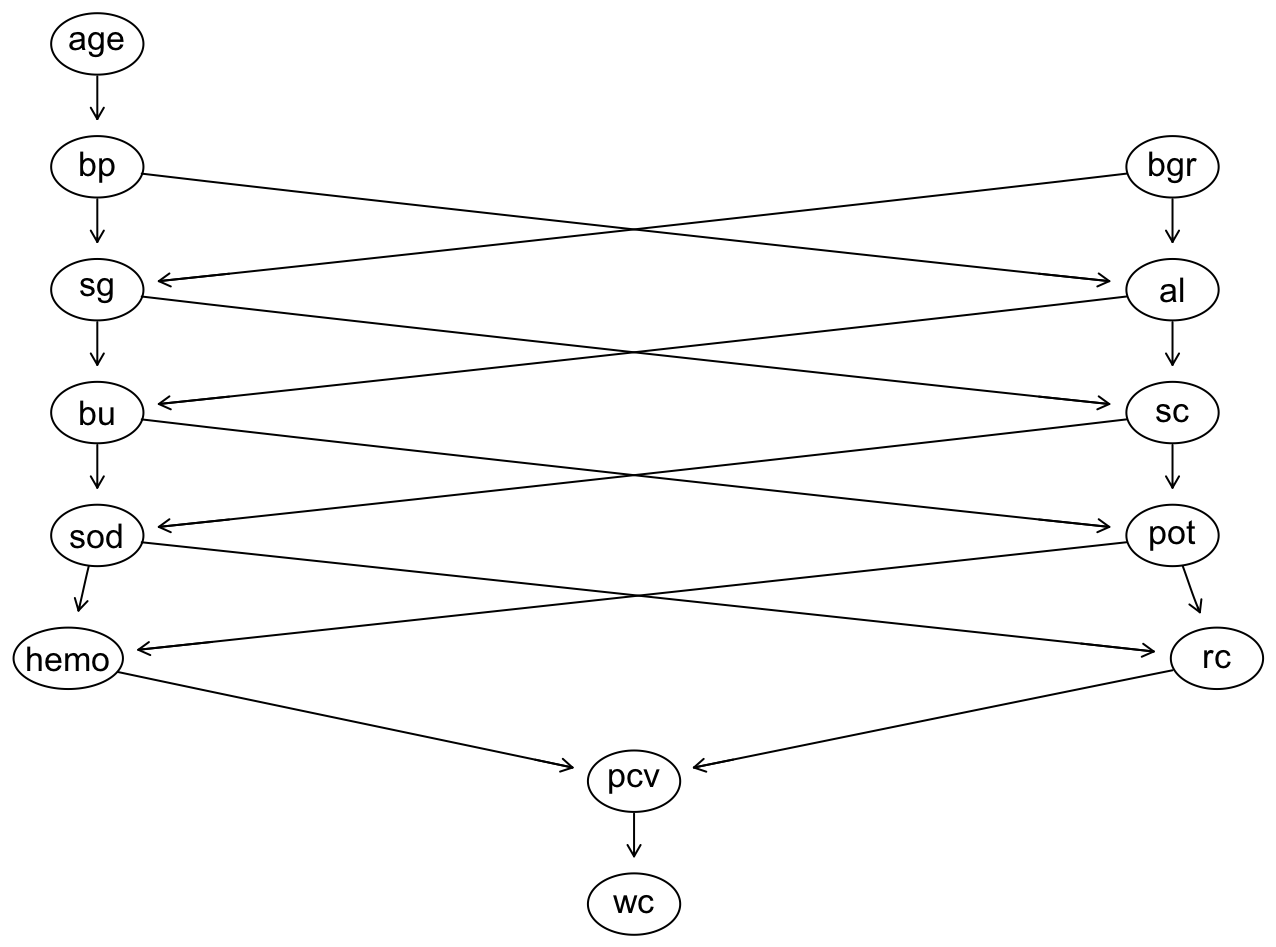
\includegraphics[width=\textwidth]{figs/dag1.png}
\caption{\textbf{DAG 1} (estudiante de 5º semestre) --- la ERC como cascada estricta; la anemia
cuelga de los electrolitos.}
\label{fig:dag1}
\end{figure}

\begin{figure}[htbp]
\centering
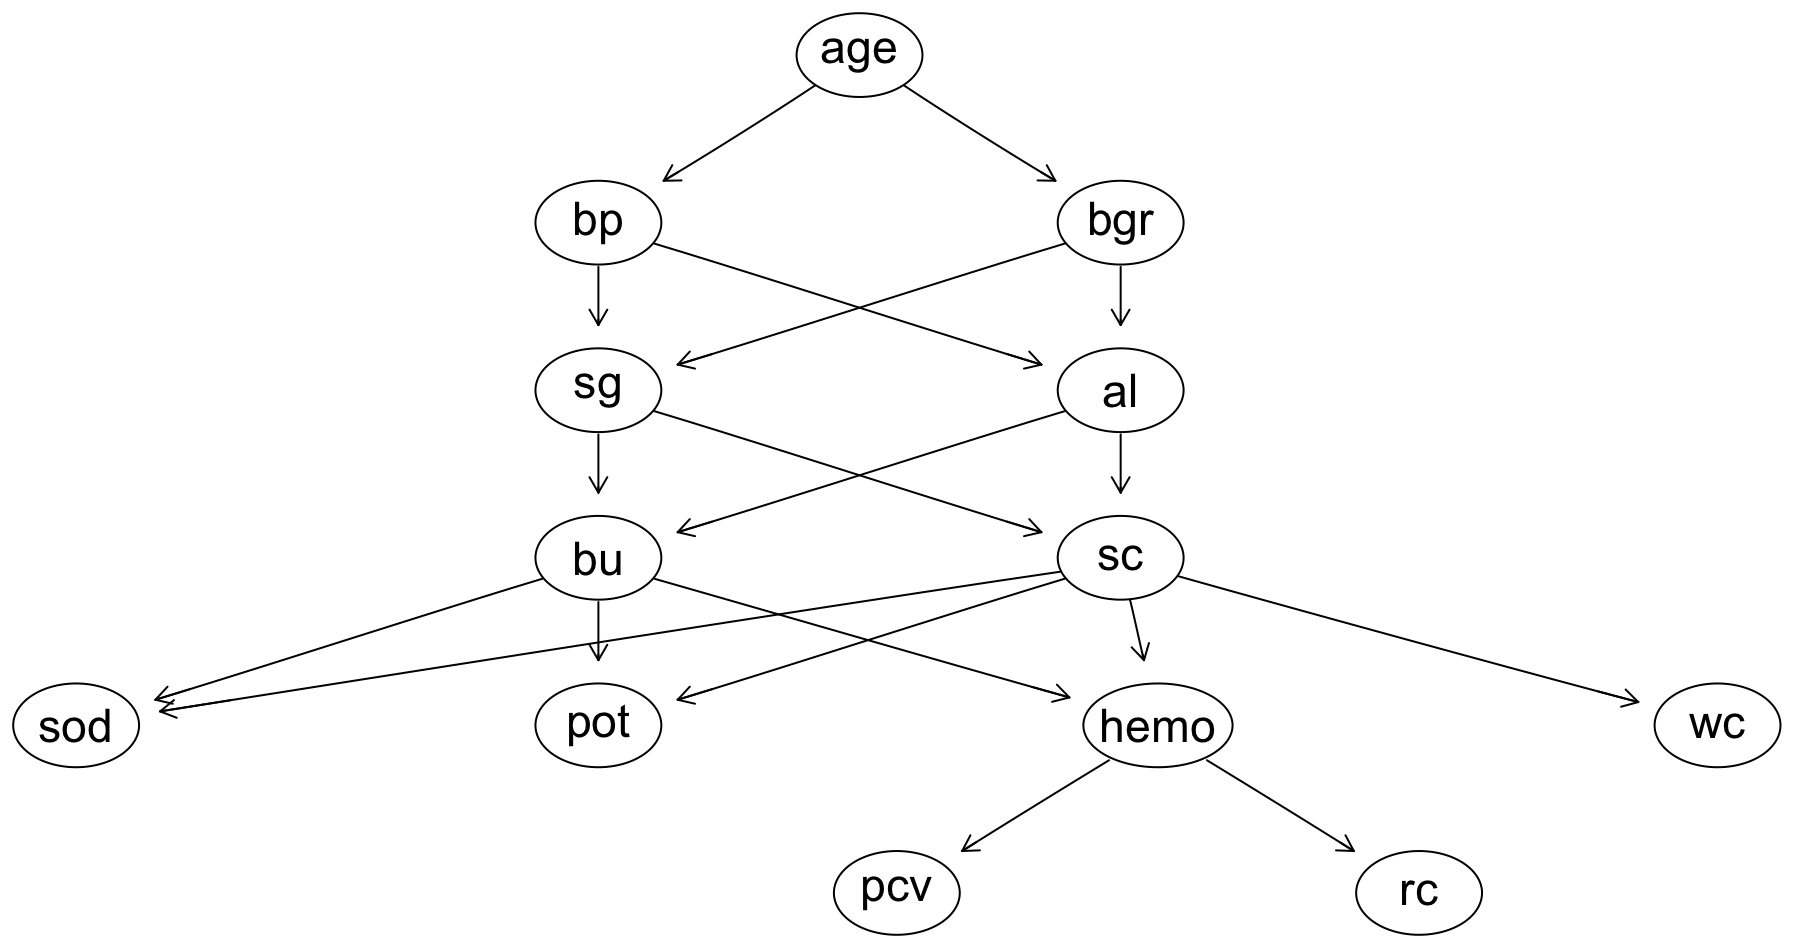
\includegraphics[width=\textwidth]{figs/dag2.png}
\caption{\textbf{DAG 2} (9º semestre, A) --- la edad como origen de las dos causas principales y
la anemia colgando de los marcadores de filtrado. Es la estructura seleccionada por BIC y AIC.}
\label{fig:dag2}
\end{figure}

\begin{figure}[htbp]
\centering
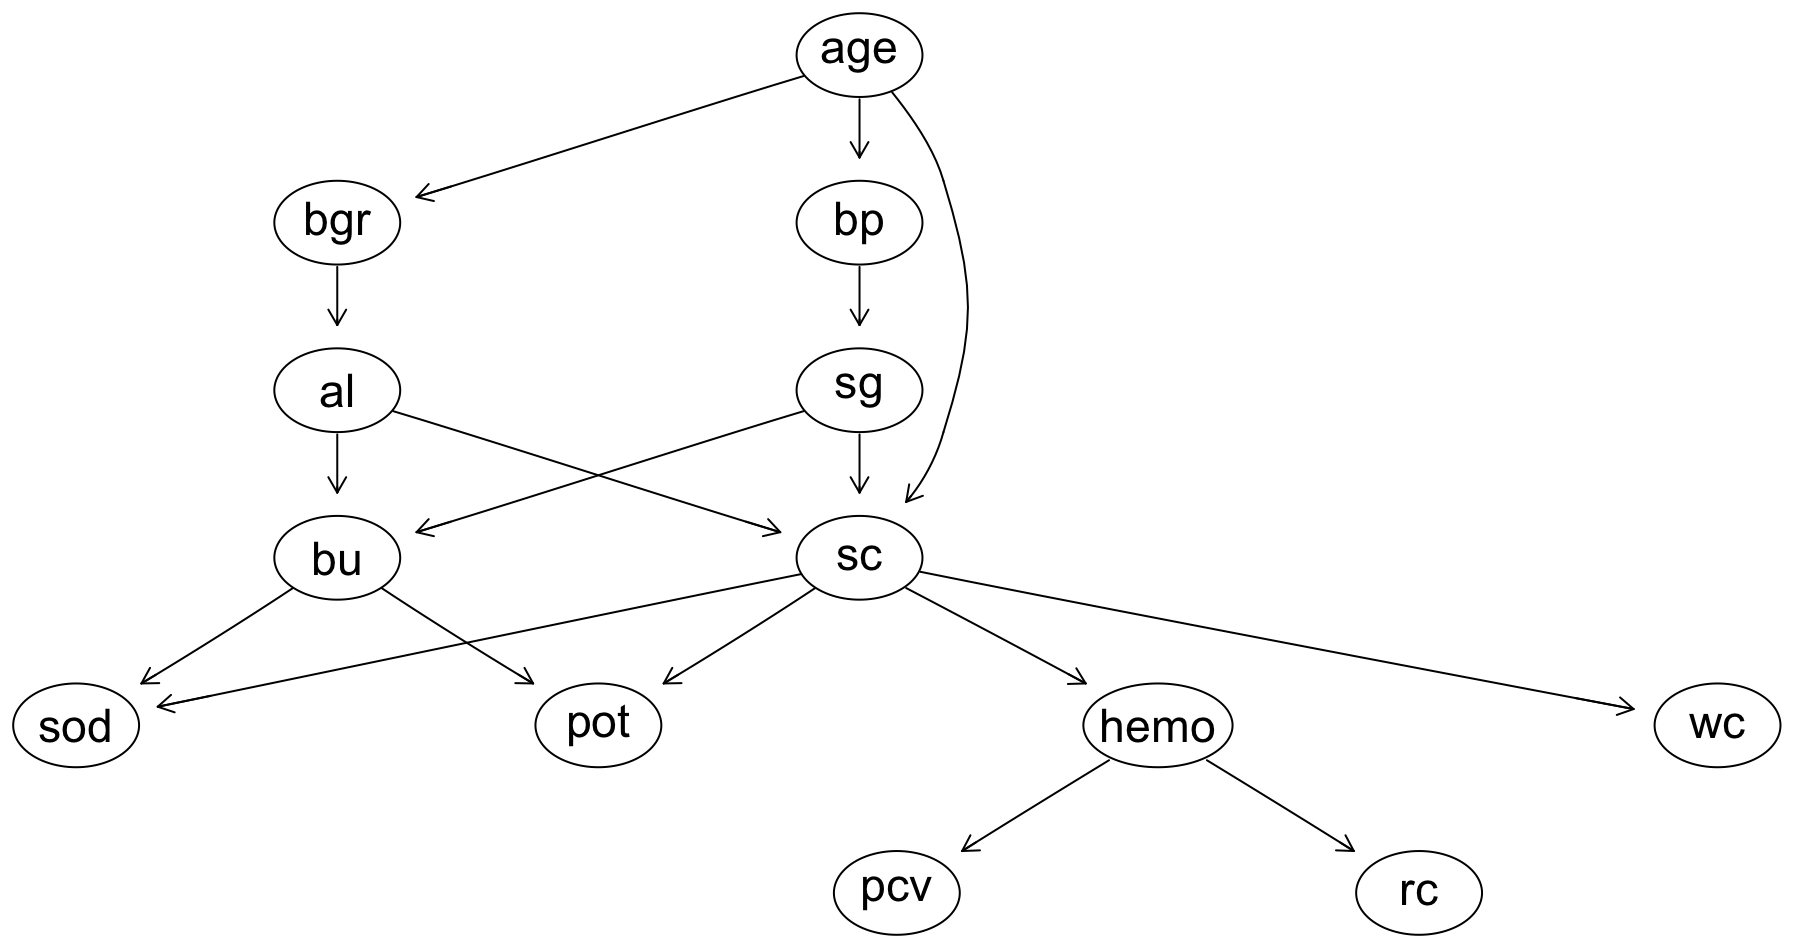
\includegraphics[width=\textwidth]{figs/dag3.png}
\caption{\textbf{DAG 3} (9º semestre, B) --- dos vías de daño separadas, glomerular y tubular, que
convergen en los marcadores de filtrado.}
\label{fig:dag3}
\end{figure}

\begin{table}[H]
\centering
\caption{Comparación estructural de las tres propuestas. Los conteos $tp/fp/fn$ y la distancia
estructural (SHD) toman la DAG 1 como referencia.}
\label{tab:estructuras}
\small
\renewcommand{\arraystretch}{1.12}
\begin{tabular}{l c c c c c c}
\toprule
\textbf{Estructura} & \textbf{Arcos} & \textbf{Acíclica} & \textbf{$tp$} & \textbf{$fp$} &
\textbf{$fn$} & \textbf{SHD vs.\ DAG 1} \\
\midrule
DAG 1 (5º sem)    & 20 & sí & --- & --- & --- & --- \\
DAG 2 (9º sem A)  & 19 & sí & 14 & 5 & 6 & 11 \\
DAG 3 (9º sem B)  & 17 & sí & 12 & 5 & 8 & 15 \\
\midrule
\multicolumn{7}{l}{\footnotesize SHD entre las dos propuestas de 9º semestre: \textbf{6}.}\\
\bottomrule
\end{tabular}
\end{table}

Las tres coinciden en la parte inicial de la cascada —la DAG 2 comparte 14 de los 20 arcos de la
DAG 1 y la DAG 3 comparte 12— y se separan en el tramo final: en cómo llega el daño renal a la
anemia. Las dos propuestas de 9º semestre son las más parecidas entre sí (SHD $=6$), lo que
sugiere que la formación adicional converge hacia una misma lectura del mecanismo.

\subsection{Ajuste y comparación de las tres redes}

Se ajustó una GBN por estructura sobre las 400 observaciones imputadas. La
Tabla~\ref{tab:scores} reporta ambos criterios.

\begin{table}[H]
\centering
\caption{Comparación de las tres GBN sobre las 400 observaciones imputadas. Valores mayores
indican mejor ajuste. La última columna es una reproducción independiente del BIC, implementada
desde cero en Python.}
\label{tab:scores}
\small
\renewcommand{\arraystretch}{1.15}
\begin{tabular}{l c r r r}
\toprule
\textbf{Estructura} & \textbf{Arcos} & \textbf{BIC} & \textbf{AIC} & \textbf{BIC (verif.)} \\
\midrule
DAG 1 (5º sem)   & 20 & $-16{,}620.07$ & $-16{,}528.26$ & $-16{,}620.01$ \\
DAG 2 (9º sem A) & 19 & $\mathbf{-16{,}374.23}$ & $\mathbf{-16{,}284.42}$ & $-16{,}374.18$ \\
DAG 3 (9º sem B) & 17 & $-16{,}453.82$ & $-16{,}368.00$ & $-16{,}453.77$ \\
\bottomrule
\end{tabular}
\end{table}

Los dos criterios coinciden en el orden, lo que hace la conclusión robusta: la \textbf{DAG 2} es
la mejor, seguida de la DAG 3 y al final la DAG 1. La ventaja de la DAG 2 sobre la DAG 1 es de
\textbf{245.8 puntos de BIC} y sobre la DAG 3 de 79.6, distancias que no dejan lugar a la duda —a
diferencia de lo que ocurre cuando dos estructuras difieren en unas pocas unidades—. Como
verificación, los tres puntajes se recalcularon implementando \eqref{eq:bic} desde cero en Python
a partir de las regresiones nodo por nodo; las diferencias con \texttt{bnlearn} son menores a
$0.07$ puntos, atribuibles al redondeo en la estimación de las desviaciones residuales.

Lo que decide la comparación es exactamente el punto en que las estructuras discrepan: dónde
cuelga la anemia. La DAG 1 la hace depender del sodio y el potasio; las DAG 2 y 3, de la
creatinina y la urea. \textbf{Los datos favorecen la segunda opción}, que es también la que la
fisiología respalda: la eritropoyetina se produce en el riñón y su caída acompaña al deterioro del
filtrado, no al desbalance electrolítico \cite{babitt2012}. Es un caso en que el criterio
estadístico y el argumento clínico apuntan en la misma dirección.

\subsection{Fuerza de los arcos}

La Tabla~\ref{tab:arcstrength} reporta \texttt{arc.strength} sobre la DAG 1 con criterio
\texttt{bic-g}, es decir, el cambio en el BIC si cada arco se eliminara.

\begin{table}[H]
\centering
\caption{Fuerza de los arcos de la DAG 1 (cambio en BIC al eliminar el arco). Valores negativos
indican que los datos sostienen el arco; el único positivo sobra.}
\label{tab:arcstrength}
\small
\setlength{\tabcolsep}{5pt}
\renewcommand{\arraystretch}{1.08}
\begin{tabular}{l l r c l l r}
\toprule
\textbf{Desde} & \textbf{Hacia} & \textbf{Fuerza} & \phantom{x} &
\textbf{Desde} & \textbf{Hacia} & \textbf{Fuerza} \\
\midrule
\texttt{sc}   & \texttt{sod}  & $-145.68$ & & \texttt{bu}   & \texttt{sod}  & $-13.67$ \\
\texttt{hemo} & \texttt{pcv}  & $-124.01$ & & \texttt{pot}  & \texttt{rc}   & $-10.79$ \\
\texttt{al}   & \texttt{bu}   & $-28.42$  & & \texttt{pot}  & \texttt{hemo} & $-7.09$  \\
\texttt{bu}   & \texttt{pot}  & $-24.37$  & & \texttt{sg}   & \texttt{sc}   & $-4.49$  \\
\texttt{sod}  & \texttt{hemo} & $-24.08$  & & \texttt{pcv}  & \texttt{wc}   & $-3.22$  \\
\texttt{bgr}  & \texttt{al}   & $-22.44$  & & \texttt{bp}   & \texttt{sg}   & $-2.40$  \\
\texttt{rc}   & \texttt{pcv}  & $-22.11$  & & \texttt{age}  & \texttt{bp}   & $-2.07$  \\
\texttt{sod}  & \texttt{rc}   & $-21.53$  & & \texttt{bp}   & \texttt{al}   & $-0.69$  \\
\texttt{bgr}  & \texttt{sg}   & $-20.16$  & & \texttt{sg}   & \texttt{bu}   & $-0.39$  \\
\texttt{al}   & \texttt{sc}   & $-20.05$  & & \texttt{sc}   & \texttt{pot}  & $\mathbf{+0.24}$ \\
\bottomrule
\end{tabular}
\end{table}

Diecinueve de los veinte arcos tienen fuerza negativa: los datos los sostienen. El único con signo
positivo es $\texttt{sc} \rightarrow \texttt{pot}$, de modo que la DAG 1 mejoraría —marginalmente,
$0.24$ puntos— si se quitara. Los dos arcos más fuertes, $\texttt{sc} \rightarrow \texttt{sod}$
($-145.7$) y $\texttt{hemo} \rightarrow \texttt{pcv}$ ($-124.0$), reflejan las dos asociaciones más
intensas del conjunto: la correlación entre creatinina y sodio es de $-0.72$ y la de hemoglobina
con hematocrito, de $0.90$. Esta última merece una advertencia: hemoglobina, hematocrito y
eritrocitos miden prácticamente lo mismo, y un arco muy fuerte entre ellos habla más de
redundancia que de mecanismo.

\subsection{Parámetros de la red elegida}

En una GBN cada nodo es una regresión, así que los parámetros se leen directamente. Dos ejemplos de
la DAG 2 ajustada:
\begin{align}
    \texttt{sc} &= 203.487 - 198.667\,\texttt{sg} + 1.475\,\texttt{al}, & \sigma &= 4.923;
    \label{eq:sc}\\
    \texttt{hemo} &= 14.352 - 0.0326\,\texttt{bu} - 0.0096\,\texttt{sc}, & \sigma &= 2.228.
    \label{eq:hemo}
\end{align}

La ecuación \eqref{eq:sc} es coherente con la clínica: la creatinina sube cuando la densidad
urinaria baja —el riñón pierde capacidad de concentrar— y sube con la albuminuria. La
\eqref{eq:hemo} anticipa un problema que reaparecerá en la consulta 3: el coeficiente de la
creatinina sobre la hemoglobina es de apenas $-0.0096$ por mg/dL, casi nulo, de modo que en el
modelo la creatinina prácticamente no mueve la hemoglobina. El ajuste completo explica el 35.5\,\%
de la varianza de la hemoglobina.

\subsection{Variables categóricas en la red}
\label{sec:categoricas}

\subsubsection*{3.6.1 La diabetes como nodo discreto}

Para responder la consulta 6 se extendió la DAG 2 con un nodo discreto, la diabetes
(\texttt{dm}: 261 pacientes sin, 137 con), colocado como padre de la glucosa. El ajuste con
\texttt{mle-cg} produce una densidad condicional distinta por nivel del padre discreto:

\begin{center}\small
\begin{tabular}{l r r}
\toprule
\textbf{\texttt{bgr} $\mid$ \texttt{dm} + \texttt{age}} & \textbf{\texttt{dm} = no} & \textbf{\texttt{dm} = sí} \\
\midrule
Intercepto                 &  96.05 & 225.41 \\
Coeficiente de \texttt{age} &   0.51 &  $-0.36$ \\
Desv.\ residual            &  39.15 &  96.07 \\
\bottomrule
\end{tabular}
\end{center}

La glucosa queda con una media muy distinta según el diagnóstico de diabetes, que es justo lo que
se buscaba, y con una dispersión residual más del doble en el grupo diabético. La restricción del
formalismo se verificó empíricamente: al intentar el arco inverso
$\texttt{wc} \rightarrow \texttt{dm}$ —un nodo discreto con padre continuo— el ajuste falla con
\textit{``arc \texttt{wc} $\rightarrow$ \texttt{dm} violates the assumptions of the model''}. Esto
tiene una consecuencia concreta sobre la DAG 1, que terminaba en
$\texttt{wc} \rightarrow \texttt{classification}$: con esa orientación el diagnóstico no puede
entrar a la red, y habría que invertir el arco y tratarlo como causa de los hallazgos y no como su
consecuencia.

\subsubsection*{3.6.2 ¿Dónde conviene colocar la diabetes?}

El especialista la puso como padre de la glucosa por razones clínicas. Para contrastar esa
decisión con los datos se evaluaron varias posiciones con el BIC condicional gaussiano sobre los
398 pacientes con \texttt{dm} registrada, tomando como referencia el modelo en que \texttt{dm}
entra a la red pero sin arcos (Tabla~\ref{tab:dm}). Como todos los modelos comparten las mismas
variables y las mismas filas, los puntajes son comparables entre sí.

\begin{table}[H]
\centering
\caption{Dónde colocar la diabetes: BIC condicional gaussiano ($n = 398$) según los nodos
continuos de los que \texttt{dm} es padre.}
\label{tab:dm}
\small
\renewcommand{\arraystretch}{1.12}
\begin{tabular}{l r r}
\toprule
\textbf{Posición de \texttt{dm}} & \textbf{BIC} & \textbf{Ganancia} \\
\midrule
Sin arcos (nodo aislado)                                        & $-16{,}557.8$ & --- \\
$\texttt{dm} \rightarrow \texttt{bp}$                           & $-16{,}547.9$ & $+9.9$   \\
$\texttt{dm} \rightarrow \texttt{sc}$                           & $-16{,}539.3$ & $+18.5$  \\
$\texttt{dm} \rightarrow \texttt{bgr}$ \textit{(propuesta del especialista)} & $-16{,}437.8$ & $+120.0$ \\
$\texttt{dm} \rightarrow \{\texttt{bgr},\texttt{bp}\}$          & $-16{,}427.9$ & $+129.9$ \\
$\texttt{dm} \rightarrow \{\texttt{bgr},\texttt{sc}\}$          & $-16{,}419.2$ & $+138.5$ \\
$\texttt{dm} \rightarrow \{\texttt{bgr},\texttt{bp},\texttt{sc}\}$ & $-16{,}409.4$ & $+148.4$ \\
Búsqueda voraz: \texttt{dm} padre de los 13 nodos               & $-16{,}207.0$ & $+350.7$ \\
\bottomrule
\end{tabular}
\end{table}

La lectura tiene dos capas. La primera confirma al especialista: de todas las posiciones
individuales, \textbf{la glucosa es con mucho la mejor} ($+120.0$ puntos, frente a $+18.5$ de la
creatinina y $+9.9$ de la presión). El arco que la clínica dictaba es también el que los datos
prefieren.

La segunda es una advertencia. Una búsqueda voraz sin restricciones termina colgando la diabetes
de \textbf{los trece nodos}, con una ganancia de $350.7$ puntos, y eso no debe leerse como que la
diabetes causa todo el cuadro. En este dataset \textbf{los 137 pacientes diabéticos son, sin
excepción, pacientes con ERC} —el análisis exploratorio encontró lo mismo en las diez variables
binarias: su nivel positivo corresponde al 100\,\% de enfermos—, y como el 54.8\,\% de los enfermos
son diabéticos, \texttt{dm} funciona como un \textbf{sustituto parcial del diagnóstico}. El
algoritmo no está descubriendo fisiología, está reencontrando la etiqueta que se le quitó a la
red. Conviene, por tanto, fijar la posición de la variable discreta por criterio clínico y usar el
puntaje solo para confirmarla.

\subsubsection*{3.6.3 El diagnóstico como raíz discreta}

El caso límite del razonamiento anterior es meter el propio diagnóstico como nodo discreto raíz,
padre de las 13 variables continuas. Bajo \eqref{eq:clgbn} esto equivale a ajustar
\textbf{dos redes gaussianas}, una por grupo, y es la formalización natural de la conjetura del
análisis exploratorio: si la no normalidad viene de mezclar enfermos y sanos, el modelo debería
mezclarlos explícitamente.

El resultado es el mayor salto de ajuste de todo el estudio: el BIC pasa de $-16{,}374.2$ a
$\mathbf{-14{,}486.5}$, una ganancia de \textbf{1{,}887.7 puntos} a cambio de duplicar los
parámetros (de 45 a 90). La ganancia no se reparte por igual: la Tabla~\ref{tab:estratif} muestra
qué nodos la piden.

\begin{table}[H]
\centering
\caption{Ganancia en BIC al estratificar cada nodo por diagnóstico (una regresión por grupo en
lugar de una común).}
\label{tab:estratif}
\small
\setlength{\tabcolsep}{4.5pt}
\begin{tabular}{l r l r l r l r}
\toprule
\textbf{Nodo} & \textbf{$\Delta$BIC} & \textbf{Nodo} & \textbf{$\Delta$BIC} &
\textbf{Nodo} & \textbf{$\Delta$BIC} & \textbf{Nodo} & \textbf{$\Delta$BIC} \\
\midrule
\texttt{al}   & $+592.9$ & \texttt{bgr}  & $+159.4$ & \texttt{bu}  & $+135.6$ & \texttt{rc}  & $+31.2$ \\
\texttt{sc}   & $+318.9$ & \texttt{hemo} & $+145.9$ & \texttt{pcv} & $+117.5$ & \texttt{sod} & $+23.4$ \\
\texttt{pot}  & $+161.5$ & \texttt{sg}   & $+144.3$ & \texttt{bp}  & $+33.4$  & \texttt{wc}  & $+18.3$ \\
              &          &               &          &              &          & \texttt{age} & $+5.4$  \\
\bottomrule
\end{tabular}
\end{table}

La albuminuria encabeza la lista por un margen enorme ($+592.9$), y la razón es la que el análisis
exploratorio ya había detectado: \textbf{ningún paciente sano presenta albúmina en orina}, de modo
que en ese grupo la variable es prácticamente una constante en cero y su varianza condicional es
minúscula. Forzar una sola gaussiana para los dos grupos es, en su caso, un error grosero. Le
siguen la creatinina, el potasio y la glucosa, los tres marcadores más asimétricos del conjunto.
Solo la edad ($+5.4$) no justifica la estratificación, lo que también tiene sentido: es la única
variable del modelo que no es una consecuencia de la enfermedad.

\subsubsection*{3.6.4 Cuánto cuesta la alternativa de discretizar}

La segunda vía —discretizar todo y ajustar una red multinomial— tiene un costo que conviene
cuantificar en lugar de mencionarlo al pasar. Al partir cada variable en tres intervalos de igual
amplitud, \texttt{sc} coloca \textbf{397 de 400 pacientes (99.2\,\%) en el primer intervalo} y
\texttt{pot} coloca 398 (99.5\,\%), dejando además un intervalo \textbf{vacío} —de ahí la
advertencia que \texttt{bnlearn} emite sobre niveles no observados—. Con esa partición, las dos
variables sobre las que giran cuatro de las seis consultas se vuelven, a efectos prácticos,
constantes. Las variables simétricas se comportan mucho mejor: \texttt{hemo} reparte 25/199/176.
La discretización por cuantiles, o con cortes clínicos —los estadios de la ERC, por ejemplo—,
sería preferible a la de igual amplitud, pero seguiría descartando la información dentro de cada
intervalo, que es justo la que las consultas de tipo $E[\cdot]$ necesitan.

\subsection{Respuesta a las consultas}

La Tabla~\ref{tab:consultas} reúne las seis respuestas junto con la frecuencia observada en los
datos sobre el mismo universo.

\begin{table}[htbp]
\centering
\caption{Respuesta a las seis consultas con la DAG 2 ajustada, frente a la evidencia observada.
La última columna reporta el mayor coeficiente de asimetría entre las variables que intervienen.}
\label{tab:consultas}
\small
\setlength{\tabcolsep}{5pt}
\renewcommand{\arraystretch}{1.15}
\begin{tabular}{l l r r r r r}
\toprule
& \textbf{Consulta} & \textbf{Red} & \textbf{Observado} & \textbf{$n$} &
\textbf{Error} & \textbf{$|$sesgo$|$} \\
\midrule
C1 & $P(\texttt{sc} > 3 \mid \texttt{bp} \geq 90)$        & 0.556  & 0.417  & 84  & $+33.3$\,\%  & 7.63 \\
C2 & $E[\texttt{pcv} \mid \texttt{hemo} < 10]$            & 27.111 & 25.848 & 75  & $+4.9$\,\%   & 0.30 \\
C3 & $E[\texttt{hemo} \mid \texttt{sc} > 5]$              & 12.072 & 8.984  & 58  & $+34.4$\,\%  & 7.63 \\
C4 & $P(\texttt{pot} > 5.5 \mid \texttt{bu} > 100)$       & 0.600  & 0.250  & 52  & $+140.0$\,\% & 12.50 \\
C5a& $E[\texttt{al} \mid \texttt{bgr} < 140]$             & 0.682  & 0.695  & 258 & $-1.9$\,\%   & 2.06 \\
C5b& $E[\texttt{al} \mid \texttt{bgr} > 200]$             & 1.711  & 2.028  & 73  & $-15.6$\,\%  & 2.06 \\
C6 & $P(\texttt{sc} > 3 \mid \texttt{dm} = \text{sí})$    & 0.561  & 0.409  & 137 & $+37.2$\,\%  & 7.63 \\
\bottomrule
\multicolumn{7}{l}{\footnotesize C6 se responde con la red gaussiana condicional; las demás, con la
GBN de la DAG 2.}\\
\end{tabular}
\end{table}

\textbf{La red acierta el sentido de las seis consultas.} La presión alta aumenta la probabilidad
de creatinina elevada (0.556 contra una marginal de 0.235); el daño renal avanzado baja la
hemoglobina; la hiperglucemia sube la albuminuria esperada, que pasa de 0.68 a 1.71; y los
pacientes diabéticos tienen más riesgo de creatinina alta. Ninguna respuesta contradice la
dirección que el especialista anticipaba al proponer la consulta.

\textbf{Las magnitudes son otra historia.} En C1, C4 y C6 la red sobreestima la probabilidad, y en
C3 no alcanza a bajar la hemoglobina tanto como lo hace el dato: predice 12.07 cuando lo observado
es 8.98, apenas $0.4$ puntos por debajo de la media marginal de 12.45. El caso extremo es C4, donde
la red duplica y media la frecuencia observada de hiperkalemia. La siguiente sección muestra que
estos errores no son aleatorios.

\subsection{Diagnóstico del supuesto gaussiano}

La Tabla~\ref{tab:normalidad} evalúa, sobre la base imputada, qué tan lejos está cada variable de
la normal que la red le impone.

\begin{table}[htbp]
\centering
\caption{Diagnóstico de normalidad sobre las 400 observaciones imputadas. SW es el $p$-valor de
la prueba de Shapiro--Wilk \cite{shapiro1965}; las dos últimas columnas reportan la asimetría dentro de cada grupo
diagnóstico.}
\label{tab:normalidad}
\small
\setlength{\tabcolsep}{5.5pt}
\renewcommand{\arraystretch}{1.1}
\begin{tabular}{l r r r r r r r}
\toprule
\textbf{Variable} & \textbf{Media} & \textbf{D.E.} & \textbf{Sesgo} & \textbf{Curtosis} &
\textbf{SW $p$} & \textbf{Sesgo \texttt{ckd}} & \textbf{Sesgo \texttt{notckd}} \\
\midrule
\texttt{age}  &   51.50 &   16.98 & $-0.68$ &   0.11 & $3\times10^{-8}$  & $-1.17$ & $0.07$ \\
\texttt{bp}   &   76.42 &   13.49 & $1.63$  &   8.85 & $8\times10^{-18}$ & $1.54$  & $-0.27$ \\
\texttt{sg}   &    1.02 &    0.01 & $-0.09$ & $-0.94$& $5\times10^{-15}$ & $0.47$  & $0.07$ \\
\texttt{al}   &    1.10 &    1.35 & $1.04$  &   0.46 & $2\times10^{-22}$ & $0.47$  & $0.22$ \\
\texttt{bgr}  &  148.45 &   75.92 & $2.06$  &   4.65 & $6\times10^{-23}$ & $1.48$  & $-0.04$ \\
\texttt{bu}   &   57.36 &   49.62 & $2.65$  &   9.52 & $3\times10^{-25}$ & $2.04$  & $-0.08$ \\
\texttt{sc}   &    3.05 &    5.62 & $7.63$  &  81.60 & $3\times10^{-34}$ & $6.38$  & $2.58$ \\
\texttt{sod}  &  137.28 &    9.94 & $-7.04$ &  84.21 & $7\times10^{-30}$ & $-7.29$ & $0.22$ \\
\texttt{pot}  &    4.55 &    2.87 & $12.50$ & 170.64 & $1\times10^{-37}$ & $10.06$ & $-0.28$ \\
\texttt{hemo} &   12.45 &    2.77 & $-0.28$ & $-0.30$& $1\times10^{-3}$  & $-0.53$ & $0.25$ \\
\texttt{pcv}  &   38.18 &    8.58 & $-0.30$ & $-0.23$& $3\times10^{-4}$  & $-0.41$ & $0.18$ \\
\texttt{wc}   & 8425.04 & 2527.65 & $1.85$  &   9.14 & $2\times10^{-17}$ & $1.92$  & $0.03$ \\
\texttt{rc}   &    4.55 &    0.94 & $0.02$  &   0.06 & $0.10$            & $0.26$  & $0.27$ \\
\bottomrule
\end{tabular}
\end{table}

El resultado es contundente: \textbf{solo 1 de las 13 variables} (\texttt{rc}) no rechaza la
normalidad al 5\,\%. El análisis exploratorio había conjeturado que el problema venía de mezclar
dos poblaciones —enfermos y sanos— y que condicionar por el diagnóstico rescataría el supuesto.
Los datos matizan esa conjetura en dos sentidos. Por un lado \textbf{la conjetura acierta en la
asimetría}: dentro del grupo sano, el sesgo de \texttt{bp} pasa de $1.63$ a $-0.27$, el de
\texttt{bu} de $2.65$ a $-0.08$, el de \texttt{sod} de $-7.04$ a $0.22$ y el de \texttt{pot} de
$12.50$ a $-0.28$; separar los grupos elimina casi toda la asimetría global. Por otro lado
\textbf{el rechazo formal persiste}: dentro de \texttt{ckd} ninguna de las 13 pasa la prueba, y
dentro de \texttt{notckd} solo una. Dos razones lo explican: la creatinina sigue fuertemente
asimétrica incluso entre sanos (sesgo $2.58$), y varias de las supuestas continuas son en realidad
ordinales o redondeadas —\texttt{bp} en múltiplos de 10, \texttt{sg} en cinco niveles, \texttt{al}
en seis—, de modo que la prueba las rechaza por los empates, no por las colas.

\textbf{El supuesto y el error van juntos.} Al cruzar el error relativo de cada consulta
(Tabla~\ref{tab:consultas}) con el mayor coeficiente de asimetría entre las variables que
intervienen, la relación es monótona y fuerte: $\rho_{\text{Spearman}} = 0.898$ con $p = 0.006$.
La consulta más precisa, C2, involucra hemoglobina y hematocrito, las dos variables mejor
comportadas (sesgo $\approx 0.3$), y yerra por 4.9\,\%. La menos precisa, C4, involucra al potasio,
con sesgo $12.50$ y curtosis $170.6$, y yerra por 140\,\%.

\textbf{Por qué falla la consulta 3.} Vale la pena desarmar un caso porque el mecanismo es
instructivo y no es el que uno supondría. La ecuación \eqref{eq:hemo} no es la culpable: evaluada
en los valores que realmente presenta el grupo con creatinina mayor a 5
($\overline{\texttt{bu}} = 143.6$, $\overline{\texttt{sc}} = 11.83$), predice una hemoglobina de
\textbf{9.56}, muy cerca del 8.98 observado. El problema está en el paso anterior. Bajo normalidad
conjunta, condicionar sobre $\texttt{sc} > 5$ implica
$E[\texttt{sc} \mid \texttt{sc} > 5] = 8.85$ y arrastra la urea solo hasta
$E[\texttt{bu} \mid \texttt{sc} > 5] = 87.6$, cuando el grupo real promedia $143.6$. Con esos
valores atenuados, la misma ecuación devuelve $11.41$ —esencialmente lo que la red reporta—. Es
decir: \textbf{la gaussiana no subestima la relación entre creatinina y hemoglobina; subestima
cuánto se acompañan las colas entre sí}. En un paciente con daño renal avanzado, la urea no sube
"lo que la correlación lineal predice", sube mucho más, y esa co-ocurrencia de extremos es
precisamente lo que una normal multivariada no puede representar.

\subsection{¿Mejoran los modelos no paramétricos el BIC y el AIC?}
\label{sec:noparam}

Con el supuesto gaussiano documentado como violado, la pregunta natural es si relajarlo mejora el
ajuste. Se ajustaron nueve variantes de la DAG 2, todas sobre las mismas 400 observaciones y todas
con la verosimilitud expresada \textbf{en la escala original} de los datos, combinando tres
ingredientes: una transformación monótona de las marginales (Yeo--Johnson con $\lambda$ estimado
por máxima verosimilitud, o el caso particular $\lambda = 0$, que es $\log(1+x)$), la
estratificación por diagnóstico de \S3.6.3, y la sustitución de la densidad normal de los residuos
por un estimador kernel. La Tabla~\ref{tab:noparam} reúne los resultados.

\begin{table}[htbp]
\centering
\caption{Nueve variantes de la DAG 2. La verosimilitud está expresada en la escala original de los
datos (con corrección jacobiana donde aplica). CV-5 es la log-verosimilitud fuera de muestra en
cinco particiones. Los conteos de parámetros marcados con $^{*}$ son nominales: no cuentan la
flexibilidad real del estimador kernel.}
\label{tab:noparam}
\small
\setlength{\tabcolsep}{5pt}
\renewcommand{\arraystretch}{1.15}
\begin{tabular}{l l r r r r r}
\toprule
& \textbf{Modelo} & \textbf{Par.} & \textbf{$\log \hat{L}$} & \textbf{BIC} & \textbf{AIC} &
\textbf{CV-5} \\
\midrule
M0 & GBN gaussiana (línea base)          & 45  & $-16{,}239.4$ & $-16{,}374.2$ & $-16{,}284.4$ & $-16{,}559.2$ \\
M1 & \; + Yeo--Johnson                    & 58  & $-14{,}767.3$ & $-14{,}941.1$ & $-14{,}825.3$ & $-15{,}034.6$ \\
M2 & \; + estratificada por diagnóstico   & 90  & $-14{,}216.8$ & $-14{,}486.5$ & $-14{,}306.8$ & $-14{,}592.4$ \\
M3 & \; Yeo--Johnson + estratificada      & 103 & $-13{,}595.4$ & $-13{,}904.0$ & $-13{,}698.4$ & $\mathbf{-14{,}014.9}$ \\
\midrule
M4 & KDE en los residuos                  & 45$^{*}$  & $-15{,}442.3$ & $-15{,}577.1$ & $-15{,}487.3$ & $-16{,}472.5$ \\
M5 & \; Yeo--Johnson + KDE                & 58$^{*}$  & $-14{,}425.5$ & $-14{,}599.2$ & $-14{,}483.5$ & $-16{,}397.0$ \\
M6 & \; YJ + estratificada + KDE          & 103$^{*}$ & $-12{,}445.6$ & $\mathbf{-12{,}754.2}$ & $\mathbf{-12{,}548.6}$ & $-13{,}810.3$ \\
\midrule
L1 & $\log(1+x)$                          & 45  & $-15{,}476.5$ & $-15{,}611.3$ & $-15{,}521.5$ & $-16{,}952.5$ \\
L3 & $\log(1+x)$ + estratificada          & 90  & $-14{,}050.0$ & $-14{,}319.6$ & $-14{,}140.0$ & $-15{,}357.7$ \\
\bottomrule
\end{tabular}
\end{table}

\textbf{Sí mejora, y por mucho, pero no por donde uno esperaría.} Los dos ingredientes que
producen ganancias grandes y \textbf{consistentes en los tres criterios} son paramétricos o
semiparamétricos, no no paramétricos: transformar las marginales aporta $+1{,}433$ puntos de BIC y
$+1{,}525$ de verosimilitud fuera de muestra sobre la línea base; estratificar por diagnóstico
aporta $+1{,}888$ y $+1{,}967$; y juntos (M3) suman $\mathbf{+2{,}470}$ de BIC y $+2{,}544$ de
CV. Que las tres medidas coincidan es lo que hace creíble la mejora.

\textbf{El estimador kernel es otra historia, y es la parte instructiva.} Por BIC nominal, M6 es el
mejor modelo de la tabla por un margen amplio ($-12{,}754.2$, es decir $+3{,}620$ sobre la línea
base). Pero ese número \textbf{no es comparable}, por la razón anticipada en \S2.8: la penalización
del BIC cuenta 103 parámetros cuando un estimador kernel con 400 observaciones tiene muchos más
grados de libertad efectivos. Al medir fuera de muestra, la ventaja se desinfla: M6 supera a M3 por
apenas $205$ puntos de CV, contra los $1{,}150$ que sugería el BIC. Y en las otras dos
comparaciones el kernel directamente \textbf{pierde}: M4 mejora el BIC en $797$ puntos sobre M0
pero solo $87$ en validación cruzada, y M5 mejora el BIC en $342$ puntos sobre M1 mientras
\textbf{empeora} la validación cruzada en $1{,}362$. La razón de esa fragilidad es la esperable en
un estimador local: una observación de prueba que cae lejos de todos los residuos de entrenamiento
recibe una densidad casi nula y aporta una log-verosimilitud enormemente negativa, algo que la
cola gaussiana —por gruesa que sea— nunca hace.

Vale la pena mirar de dónde venía la ganancia aparente del kernel. Nodo por nodo, sobre los datos
sin transformar se concentra en \texttt{pot} ($+230$), \texttt{sc} ($+142$), \texttt{bgr} ($+125$)
y \texttt{al} ($+89$), y es \textbf{negativa} en los nodos bien comportados (\texttt{rc},
\texttt{hemo}). Es decir: el kernel no está capturando una no linealidad clínica, está
absorbiendo colas extremas y \textbf{átomos} —el cero de la albuminuria, los múltiplos de 10 de la
presión—. Después de transformar las marginales, la única ganancia que sobrevive con claridad
sigue siendo la de \texttt{pot} ($+187$) y la de \texttt{al} ($+71$), las dos variables con masa
puntual. La conclusión es que buena parte de lo que aquí parecía ``no normalidad'' es en realidad
\textbf{discretitud}, y el remedio adecuado para eso no es un kernel sino declarar esas variables
como lo que son —ordinales— dentro de una red mixta.

\subsubsection*{3.9.1 Un modelo utilizable: transformación logarítmica y estratificación}

M3 es el mejor modelo por verosimilitud, pero tiene un defecto que solo aparece al usarlo. Los
$\lambda$ estimados son negativos en seis variables (\texttt{sc}: $-0.95$; \texttt{bp} y
\texttt{al}: $-0.68$; \texttt{bgr}: $-0.41$), y una transformación de Yeo--Johnson con
$\lambda < 0$ tiene \textbf{soporte acotado}: la transformada inversa
$x = (\lambda z + 1)^{1/\lambda} - 1$ tiene una asíntota vertical en $z = -1/\lambda$. La gaussiana
del espacio transformado no respeta esa cota, así que al simular aparecen valores devueltos
astronómicos. En la práctica esto arruina las consultas sobre albuminuria: M3 estima
$E[\texttt{al} \mid \texttt{bgr} < 140] = 11.1$ cuando lo observado es $0.695$. \textbf{El mejor
modelo de densidad no es automáticamente el mejor simulador.}

La corrección es fijar $\lambda = 0$, es decir usar $\log(1+x)$, que es monótona, de soporte no
acotado y —al no estimarse— \textbf{no consume parámetros}. El modelo resultante, L3, mejora el
BIC en $\mathbf{+2{,}054.6}$ puntos y la validación cruzada en $+1{,}201.5$ respecto de la línea
base, y sí se puede simular. La Tabla~\ref{tab:consultas-l3} rehace las consultas con él.

\begin{table}[H]
\centering
\caption{Las consultas respondidas con la GBN gaussiana original (M0) y con el modelo
$\log(1+x)$ + estratificado (L3), por muestreo directo de $4\times10^{5}$ realizaciones.}
\label{tab:consultas-l3}
\small
\setlength{\tabcolsep}{4.5pt}
\renewcommand{\arraystretch}{1.15}
\begin{tabular}{l l r r r r r}
\toprule
& \textbf{Consulta} & \textbf{Obs.} & \textbf{M0} & \textbf{L3} &
\textbf{Err.\ M0} & \textbf{Err.\ L3} \\
\midrule
C1  & $P(\texttt{sc} > 3 \mid \texttt{bp} \geq 90)$   & 0.417  & 0.558  & 0.463  & 33.9\,\%  & \textbf{11.2\,\%} \\
C2  & $E[\texttt{pcv} \mid \texttt{hemo} < 10]$       & 25.848 & 27.088 & 26.656 & 4.8\,\%   & \textbf{3.1\,\%}  \\
C3  & $E[\texttt{hemo} \mid \texttt{sc} > 5]$         & 8.984  & 12.066 & 10.266 & 34.3\,\%  & \textbf{14.3\,\%} \\
C4  & $P(\texttt{pot} > 5.5 \mid \texttt{bu} > 100)$  & 0.250  & 0.599  & 0.546  & 139.6\,\% & \textbf{118.3\,\%}\\
C5a & $E[\texttt{al} \mid \texttt{bgr} < 140]$        & 0.695  & 0.686  & 0.680  & \textbf{1.3\,\%} & 2.2\,\% \\
C5b & $E[\texttt{al} \mid \texttt{bgr} > 200]$        & 2.028  & 1.705  & 2.033  & 15.9\,\%  & \textbf{0.3\,\%}  \\
\midrule
    & \textbf{Error relativo medio}                   &        &        &        & \textbf{38.3\,\%} & \textbf{24.9\,\%} \\
\bottomrule
\multicolumn{7}{@{}p{14.6cm}@{}}{\footnotesize La columna M0 reproduce, mediante un muestreador
propio, los valores que \texttt{cpquery} entrega en la Tabla~\ref{tab:consultas}: 0.558 contra
0.556, 27.088 contra 27.111, 12.066 contra 12.072 y 0.599 contra 0.600. La diferencia es ruido de
muestreo.}\\
\end{tabular}
\end{table}

El error relativo medio baja de $38.3$\,\% a $24.9$\,\%, y la mejora se concentra justo donde el
diagnóstico de \S3.8 predecía: las consultas dominadas por variables asimétricas. C1 pasa de
$33.9$\,\% a $11.2$\,\% de error, C3 de $34.3$\,\% a $14.3$\,\%, y C5b —la albuminuria bajo
hiperglucemia— pasa de $15.9$\,\% a $0.3$\,\%. La única que sigue mal es C4, la hiperkalemia, y no
sorprende: el potasio tiene un máximo de $47$ mmol/L en una escala cuyo percentil 75 es $4.9$, y
ninguna transformación monótona global reconcilia eso con una gaussiana.

\subsection{Contraste contra una estructura aprendida de los datos}

Ninguna de las tres estructuras proviene de los datos, así que como extensión de este trabajo se
ejecutó una \textbf{búsqueda voraz} (\textit{hill-climbing}) sobre los mismos 400 registros,
maximizando el BIC gaussiano de \eqref{eq:bic}, implementada desde cero para poder inspeccionar
cada paso. La red aprendida es:

\begin{quote}\footnotesize\ttfamily\raggedright
\mbox{[bgr][age|rc:bgr][bp|pcv][al|bgr][hemo|al]}\\
\mbox{[sg|hemo:sod:bgr][sod|al:bgr][bu|pcv:al:rc]}\\
\mbox{[sc|bu:sod:hemo][pot|bu:sod:sc][pcv|hemo:sg]}\\
\mbox{[rc|pcv:hemo][wc|sg]}
\end{quote}

Con 24 arcos alcanza un BIC de $-16{,}096.5$, \textbf{278 puntos por encima de la DAG 2}. Y sin
embargo no es una estructura utilizable: incluye $\texttt{rc} \rightarrow \texttt{age}$ —el conteo
de eritrocitos como causa de la edad— y $\texttt{pcv} \rightarrow \texttt{bp}$, orientaciones que
ningún clínico aceptaría. La razón es conocida: dentro de una clase de equivalencia de Markov,
varias orientaciones producen exactamente el mismo ajuste, y un criterio de \textit{score} no tiene
forma de preferir la correcta \cite{koller2009,chickering2002}.

El contraste delimita bien lo que aporta cada fuente. De los 19 arcos de la DAG 2, el algoritmo
recupera 7 con la misma orientación —entre ellos $\texttt{al} \rightarrow \texttt{bu}$,
$\texttt{bgr} \rightarrow \texttt{al}$, $\texttt{bu} \rightarrow \texttt{pot}$ y
$\texttt{hemo} \rightarrow \texttt{pcv}$— y 3 más invertidos, de modo que 10 de las 19
\textit{adyacencias} propuestas por el especialista aparecen también en la solución de los datos.
Los datos, en suma, confirman buena parte de las \textbf{conexiones} que el experto dibujó y no
sirven para decidir su \textbf{dirección}; el experto aporta exactamente lo contrario. Un
aprendizaje con lista blanca —que fije las orientaciones clínicamente indiscutibles y deje al
algoritmo el resto— es la síntesis natural de ambos.

\subsection{Limitaciones}

\textbf{El supuesto gaussiano no se cumple.} Doce de las trece variables rechazan la normalidad, y
el error de las consultas escala con la asimetría. La \S3.9 muestra que la transformación
logarítmica y la mezcla condicional recortan ese error de $38.3$\,\% a $24.9$\,\%, pero no lo
eliminan: incluso con el modelo corregido, las respuestas deben leerse como el sentido y el tamaño
relativo del efecto, no como probabilidades aplicables a un paciente concreto.

\textbf{Variables ordinales tratadas como continuas.} \texttt{bp}, \texttt{sg} y \texttt{al} tienen
10, 5 y 6 niveles observados. Además, la imputación les asigna valores intermedios que no existen
en la escala de medición.

\textbf{Imputación de punto único.} Se usó una sola realización de MICE, de modo que la
incertidumbre de la imputación no se propaga a las estimaciones. La práctica recomendada es generar
varias imputaciones y combinar los resultados con las reglas de Rubin \cite{little2002}.

\textbf{Redundancia entre variables.} \texttt{hemo}, \texttt{pcv} y \texttt{rc} correlacionan entre
$0.83$ y $0.90$: miden esencialmente lo mismo, y los arcos que los unen inflan el ajuste sin
aportar mecanismo.

\textbf{Universos pequeños en las colas.} Las consultas se evalúan sobre 52 a 84 pacientes, salvo
C5a. La frecuencia observada que sirve de referencia tiene, ella misma, un margen de error amplio.

\textbf{Un solo hospital.} Los 400 registros provienen de un mismo centro y un periodo de dos
meses; nada garantiza que los coeficientes estimados se trasladen a otra población.

% ─── 4. CONCLUSIONES ──────────────────────────────────────────────────────────
\section{Conclusiones}

\begin{enumerate}
    \item La \textbf{DAG 2}, propuesta por un estudiante de 9º semestre, es la mejor de las tres
        por ambos criterios (BIC $=-16{,}374.2$; AIC $=-16{,}284.4$), con una ventaja de 245.8
        puntos de BIC sobre la propuesta de 5º semestre. Los puntajes se verificaron con una
        implementación independiente.
    \item Lo que decide la comparación es \textbf{dónde cuelga la anemia}. Los datos favorecen
        hacerla depender de los marcadores de filtrado y no de los electrolitos, que es también lo
        que la fisiología indica: la eritropoyetina se produce en el riñón.
    \item La red \textbf{acierta el sentido de las seis consultas} y falla su magnitud. El error
        no es aleatorio: correlaciona con la asimetría de las variables implicadas
        ($\rho = 0.898$, $p = 0.006$), de 4.9\,\% en la consulta que solo involucra hemoglobina y
        hematocrito a 140\,\% en la que involucra al potasio.
    \item El mecanismo del error quedó identificado: al condicionar sobre una cola, la gaussiana
        \textbf{atenúa el co-movimiento} de las demás variables. Para la consulta 3 predice una
        urea de $87.6$ donde el grupo real promedia $143.6$; alimentada con los valores reales, la
        misma ecuación de la red acierta ($9.56$ contra $8.98$ observado).
    \item El supuesto gaussiano \textbf{no se rescata condicionando por el diagnóstico}, como el
        análisis exploratorio conjeturaba. Separar los grupos elimina casi toda la asimetría de la
        mayoría de las variables, pero solo 1 de 13 pasa Shapiro--Wilk globalmente y ninguna dentro
        del grupo enfermo.
    \item Una \textbf{búsqueda voraz} supera a las tres propuestas por 278 puntos de BIC, pero con
        orientaciones imposibles. Los datos confirman las conexiones que el experto dibujó y no
        deciden su dirección; el experto aporta justo lo contrario.
    \item La \textbf{red gaussiana condicional} resuelve la incorporación de variables categóricas
        siempre que estas no tengan padres continuos, condición que la clínica satisface de forma
        natural cuando la categórica —diabetes, diagnóstico— va al inicio de la cascada. Los datos
        \textbf{confirman la posición clínica de la diabetes}: como padre de la glucosa aporta
        $+120.0$ puntos de BIC, muy por encima de cualquier otra posición individual. Una búsqueda
        sin restricciones la cuelga de los trece nodos ($+350.7$), pero eso refleja una
        \textbf{fuga del diagnóstico} —los 137 diabéticos del dataset son todos enfermos— y no
        fisiología.
    \item Meter el \textbf{diagnóstico como raíz discreta} —equivalente a ajustar dos redes
        gaussianas, una por grupo— es la modificación más rentable de todo el estudio:
        $+1{,}887.7$ puntos de BIC. La albuminuria explica por sí sola un tercio de esa ganancia,
        porque ningún paciente sano presenta albúmina en orina y forzar una gaussiana común para
        ambos grupos es, en su caso, indefendible.
    \item Sobre los \textbf{modelos no paramétricos}: el estimador kernel mejora el BIC nominal
        hasta en $3{,}620$ puntos, pero \textbf{ese número no es comparable} —la penalización del
        BIC supone una familia paramétrica de dimensión fija—. Medido fuera de muestra el kernel
        aporta poco ($+87$ puntos sobre la línea base) y en una de las tres comparaciones
        \textbf{empeora} el ajuste en $1{,}362$ puntos. Lo que sí mejora de forma consistente en
        los tres criterios es semiparamétrico: transformar las marginales ($+1{,}433$ de BIC) y
        estratificar por diagnóstico ($+1{,}888$), que juntos suman $+2{,}470$.
    \item El modelo recomendado en la práctica es $\log(1+x)$ \textbf{más estratificación}: no
        consume parámetros adicionales, mejora el BIC en $2{,}054.6$ puntos y \textbf{reduce el
        error medio de las seis consultas de $38.3$\,\% a $24.9$\,\%}. El mejor modelo de
        densidad (Yeo--Johnson con $\lambda$ libre) no sirve para simular: con $\lambda$ negativo
        el soporte queda acotado y las muestras devueltas explotan.
    \item Un DAG \textbf{no puede representar retroalimentación}. La observación del especialista
        sobre el efecto del sodio y el potasio en la presión arterial es correcta y quedó fuera del
        modelo por ser cíclica: modelar ese lazo exige una red dinámica.
\end{enumerate}

\textbf{Trabajo futuro.} Las dos relajaciones que este trabajo probó —transformación de las
marginales y mezcla condicional al diagnóstico— dejan abiertas cuatro líneas. Primero, tratar
\texttt{bp}, \texttt{sg} y \texttt{al} como lo que son, \textbf{variables ordinales}, dentro de
una red gaussiana condicional que las coloque como nodos discretos: el análisis por nodo sugiere
que ahí está buena parte de lo que el estimador kernel absorbía. Segundo, ajustar una
\textbf{red bayesiana semiparamétrica} \cite{atienza2022}, que decide nodo por nodo entre una CPD
lineal gaussiana y una por kernel usando verosimilitud validada cruzadamente, en lugar de imponer
el mismo tipo de densidad a los trece nodos. Tercero, \textbf{imputación múltiple} con combinación
por las reglas de Rubin, para que la incertidumbre de los faltantes llegue a las respuestas.
Cuarto, \textbf{aprendizaje de estructura con lista blanca} y \textit{bootstrap} de arcos, que
combinaría el conocimiento clínico sobre la dirección con la capacidad de los datos para detectar
conexiones no anticipadas y reportaría qué tan estable es cada arco al remuestrear.

% ─── REFERENCIAS ──────────────────────────────────────────────────────────────
\begin{thebibliography}{99}
\small

\bibitem{pearl1988} Pearl, J. (1988). \textit{Probabilistic Reasoning in Intelligent Systems:
Networks of Plausible Inference}. San Mateo, CA: Morgan Kaufmann.

\bibitem{koller2009} Koller, D., \& Friedman, N. (2009). \textit{Probabilistic Graphical Models:
Principles and Techniques}. Cambridge, MA: MIT Press.

\bibitem{shachter1989} Shachter, R. D., \& Kenley, C. R. (1989). Gaussian influence diagrams.
\textit{Management Science}, 35(5), 527--550.

\bibitem{geiger1994} Geiger, D., \& Heckerman, D. (1994). Learning Gaussian networks. En
\textit{Proceedings of the 10th Conference on Uncertainty in Artificial Intelligence}, 235--243.

\bibitem{lauritzen1989} Lauritzen, S. L., \& Wermuth, N. (1989). Graphical models for associations
between variables, some of which are qualitative and some quantitative. \textit{The Annals of
Statistics}, 17(1), 31--57.

\bibitem{lauritzen1992} Lauritzen, S. L. (1992). Propagation of probabilities, means and variances
in mixed graphical association models. \textit{Journal of the American Statistical Association},
87(420), 1098--1108.

\bibitem{chickering2002} Chickering, D. M. (2002). Optimal structure identification with greedy
search. \textit{Journal of Machine Learning Research}, 3, 507--554.

\bibitem{scutari2010} Scutari, M. (2010). Learning Bayesian networks with the \texttt{bnlearn} R
package. \textit{Journal of Statistical Software}, 35(3), 1--22.

\bibitem{akaike1974} Akaike, H. (1974). A new look at the statistical model identification.
\textit{IEEE Transactions on Automatic Control}, 19(6), 716--723.

\bibitem{schwarz1978} Schwarz, G. (1978). Estimating the dimension of a model. \textit{The Annals
of Statistics}, 6(2), 461--464.

\bibitem{lucas2004} Lucas, P. J. F., van der Gaag, L. C., \& Abu-Hanna, A. (2004). Bayesian
networks in biomedicine and health-care. \textit{Artificial Intelligence in Medicine}, 30(3),
201--214.

\bibitem{kononenko2001} Kononenko, I. (2001). Machine learning for medical diagnosis: History,
state of the art and perspective. \textit{Artificial Intelligence in Medicine}, 23(1), 89--109.

\bibitem{levey2012} Levey, A. S., \& Coresh, J. (2012). Chronic kidney disease. \textit{The
Lancet}, 379(9811), 165--180.

\bibitem{babitt2012} Babitt, J. L., \& Lin, H. Y. (2012). Mechanisms of anemia in CKD.
\textit{Journal of the American Society of Nephrology}, 23(10), 1631--1634.

\bibitem{ckd2015} Rubini, L., Soundarapandian, P., \& Eswaran, P. (2015). \textit{Chronic Kidney
Disease} [Dataset]. UCI Machine Learning Repository.
\url{https://doi.org/10.24432/C5G020}

\bibitem{rubin1976} Rubin, D. B. (1976). Inference and missing data. \textit{Biometrika}, 63(3),
581--592.

\bibitem{little2002} Little, R. J. A., \& Rubin, D. B. (2002). \textit{Statistical Analysis with
Missing Data} (2a ed.). Hoboken, NJ: Wiley.

\bibitem{vanbuuren2011} van Buuren, S., \& Groothuis-Oudshoorn, K. (2011). \texttt{mice}:
Multivariate imputation by chained equations in R. \textit{Journal of Statistical Software}, 45(3),
1--67.

\bibitem{box1964} Box, G. E. P., \& Cox, D. R. (1964). An analysis of transformations.
\textit{Journal of the Royal Statistical Society, Series B}, 26(2), 211--252.

\bibitem{yeo2000} Yeo, I.-K., \& Johnson, R. A. (2000). A new family of power transformations to
improve normality or symmetry. \textit{Biometrika}, 87(4), 954--959.

\bibitem{hofmann1996} Hofmann, R., \& Tresp, V. (1996). Discovering structure in continuous
variables using Bayesian networks. En \textit{Advances in Neural Information Processing Systems},
8, 500--506.

\bibitem{atienza2022} Atienza, D., Bielza, C., \& Larrañaga, P. (2022). Semiparametric Bayesian
networks. \textit{Information Sciences}, 584, 564--582.

\bibitem{liu2009} Liu, H., Lafferty, J., \& Wasserman, L. (2009). The nonparanormal:
Semiparametric estimation of high-dimensional undirected graphs. \textit{Journal of Machine
Learning Research}, 10, 2295--2328.

\bibitem{elidan2010} Elidan, G. (2010). Copula Bayesian networks. En \textit{Advances in Neural
Information Processing Systems}, 23, 559--567.

\bibitem{moral2001} Moral, S., Rumí, R., \& Salmerón, A. (2001). Mixtures of truncated
exponentials in hybrid Bayesian networks. En \textit{Symbolic and Quantitative Approaches to
Reasoning with Uncertainty (ECSQARU)}, LNCS 2143, 156--167.

\bibitem{shenoy2011} Shenoy, P. P., \& West, J. C. (2011). Inference in hybrid Bayesian networks
using mixtures of polynomials. \textit{International Journal of Approximate Reasoning}, 52(5),
641--657.

\bibitem{silverman1986} Silverman, B. W. (1986). \textit{Density Estimation for Statistics and
Data Analysis}. Londres: Chapman \& Hall.

\bibitem{hastie2009} Hastie, T., Tibshirani, R., \& Friedman, J. (2009). \textit{The Elements of
Statistical Learning} (2a ed.). Nueva York: Springer.

\bibitem{shapiro1965} Shapiro, S. S., \& Wilk, M. B. (1965). An analysis of variance test for
normality (complete samples). \textit{Biometrika}, 52(3/4), 591--611.

\bibitem{pedregosa2011} Pedregosa, F., et al.\ (2011). Scikit-learn: Machine learning in Python.
\textit{Journal of Machine Learning Research}, 12, 2825--2830.

\bibitem{mckinney2010} McKinney, W. (2010). Data structures for statistical computing in Python.
En \textit{Proceedings of the 9th Python in Science Conference}, 56--61.

\bibitem{rcore2024} R Core Team (2024). \textit{R: A Language and Environment for Statistical
Computing}. Viena: R Foundation for Statistical Computing.

\end{thebibliography}

\end{document}
